\documentclass[a4paper,11pt, twoside]{article}

\usepackage[a4paper,top=3cm,bottom=3.5cm,left=2.5cm,right=2.5cm]{geometry}
\usepackage{graphicx}
\usepackage[utf8x]{inputenc}
\usepackage[italian]{babel}
\usepackage{fancyhdr}
\usepackage{amssymb}
\usepackage{makeidx}
\usepackage{eurosym}
\usepackage{hyperref}
\usepackage{varioref}
\usepackage{xmpincl}
\usepackage{ccicons}


\usepackage{amsthm}

\theoremstyle{definition}
\newtheorem{defn}{Definizione}[section]

\title{Appunti di Progettazione Hardware 2}
\author{Matteo Gianello}
\date{\today}

\pdfinfo{%
  /Title    (Appunti di Progettazione Hardware 2)
  /Author   (Matteo Gianello)
  /Creator  (Matteo Gianello)
  /Producer ()
  /Subject  ()
  /Keywords (Progettazione Hardware 2 Ferrandi IngInf Polimi)
}
\makeindex
\includexmp{licenza}
\begin{document}
\pagestyle{empty}
\thispagestyle{empty}
\maketitle
\vspace{5cm}
\begin{center}
Quest'opera è stata rilasciata con licenza Creative Commons Attribuzione - Non commerciale - Condividi allo stesso modo 3.0 Unported. Per leggere una copia della licenza visita il sito web \url{http://creativecommons.org/licenses/by-nc-sa/3.0/deed.it} \ccbyncsa.
\end{center}
\newpage

\thispagestyle{plain}
\tableofcontents
\newpage

\pagestyle{plain}
\section*{Introduzione}
Il corso di Architetture Avanzate dei Calcolatori si prefigge lo scopo di fornire una vista sulle più recenti architetture avanzate dei calcolatori, introducendo i meccanismi base delle micro-architetture che si possono ritrovare nei moderni microprocessori, ed infine fornire le ragioni dietro alle tecniche adottate nelle architetture dei computer.
\section{Pipelining}\label{capitolo1}
\subsection{Concetti base}
Definiamo prima di tutto quali sono le principali caratteristiche dell'architettura MIPS partendo dalla definizione delle istruzioni utilizzate da questi calcolatori calcolatori.
Esistono due tipi di istruzioni le CISC e le RISC; le istruzioni di tipo \textbf{CISC} (\emph{Complex Instruction Set Computer}) sono un set di istruzioni esteso che permettono ai processori di eseguire operazioni molto complesse come somme tra operandi caricati direttamente dalla memoria centrale, le istruzioni \textbf{RISC} (\emph{Reduced Instruction Set Computer}), invece, sono istruzioni semplici che possono essere eseguite in un unico ciclo di clock e ottimizzate per le performance sulle CPU CISC.
Le architetture RISC sono anche dette architetture di tipo \emph{LOAD/STORE}, in quanto le istruzioni non accedono direttamente ai dati in memoria ma accedono ai dati contenuti in registri del processore, solo due istruzioni permettono l'accesso alla memoria principale, queste due istruzioni sono: 
\begin{itemize}
\item \textbf{load} che carica i dati dalla memoria ai registri.
\item \textbf{store} che sposta i dati dai registri alla memoria.
\end{itemize}
Un'altra caratteristica fondamentale per le architetture RISC è l'utilizzo della \emph{Pipeline} una tecnica di ottimizzazione basata sull'esecuzione sovrapposta di molteplici istruzioni sequenziali.
\subsubsection{Reduced Instruction Set nei processori MIPS}
Vediamo ora quali sono le diverse istruzioni di tipo RISC e come sono rappresentate nel calcolatore
\paragraph{Istruzioni ALU}
Vediamo innanzitutto le istruzioni di somma ovvero quelle eseguite dalla ALU. Queste possono essere di due tipi,
Una istruzione di tipo \emph{R-Format} è un istruzione che prende in considerazione due registri, tale tipo di operazione è applicabile solo alle istruzioni \texttt{add} di tipo registro-registro. Esistono poi le \texttt{addi} che viene chiamata anche somma \emph{immediata} in quanto avviene tra un registro ed un valore costante. Tale tipo di istruzione è del tipo \emph{I-Format}.
Lo pseudo codice assembly  delle due istruzioni è mostrato qui di seguito, inoltre possiamo anche vedere come vengono svolte le operazioni.
\begin{verbatim}
add  $s1, $s2, $s3      # $s1 <- $s2 + $s3
addi $s1, $s2, 4        # $s1 <- $s2 + 4
\end{verbatim}
In \figurename\,\ref{fig:regALU} vediamo come è suddivisa un'istruzione di tipo \emph{R-Format} 
\begin{figure}[htb]
\centering
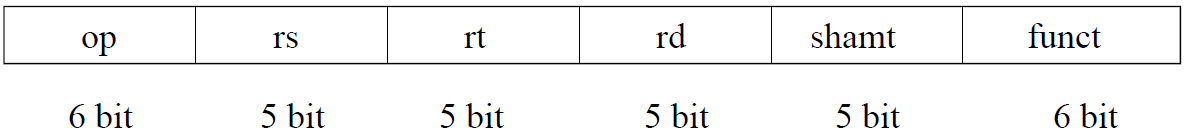
\includegraphics[scale=0.4]{img/regALU.png}
\caption{Esempio di istruzione ALU di tipo R-Format}\label{fig:regALU}
\end{figure}
I diversi campi indicano rispettivamente:
\begin{description}
\item[op] identifica il tipo di istruzione ALU da eseguire
\item[rs] indica il registro nel quale è contenuto il primo operando
\item[rt] indica il registro nel quale è contenuto il secondo operando
\item[rd] indica il registro di destinazione
\item[shamt] sta ad indicare i bit di shift amount
\item[funct] identifica i diversi tipi di istruzione
\end{description}
\begin{figure}[htb]
\centering
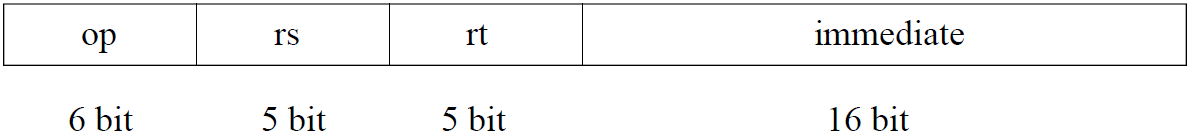
\includegraphics[scale=0.4]{img/ALUdir.png}
\caption{Divisione delle informazioni in un registro di un istruzione ALU di tipo diretto}\label{fig:ALUdir}
\end{figure}
Nella \figurename\,\ref{fig:ALUdir} vediamo invece la suddivisione di un registro nel caso di un operazione di ALU immediata.
La suddivisione dei diversi campi è la seguente:
\begin{description}
\item[op] identifica l'istruzione di tipo immediato
\item[rs] indica il registro nel quale è posizionato il primo operando
\item[rt] indica il registro di destinazione del risultato
\item[immediate] contiene il valore per l'operazione immediata nel range $-2^{15}$ e $+2^{15}-1$
\end{description}
\paragraph{Istruzioni LOAD/STORE}
Le istruzioni di \emph{load} e di \emph{store} sono quelle che permettono di caricare e scaricare i valori dai registri della CPU alla memoria centrale e viceversa.
Un esempio di codice assembly per le istruzioni load e store.
\begin{verbatim}
lw $s1, offset($s2)		# $s1 <- M[$s2 + offset]
sw $s1, offset($s2)		# M[$s2 + offset] <- $s1
\end{verbatim}
In \figurename\,\ref{fig:loadstore} vediamo come sono strutturate le istruzioni di \emph{load} e di \emph{store}; come possiamo vedere anche queste istruzioni sono nel formato \emph{I-Format}\\
\begin{figure}[htb]
\centering
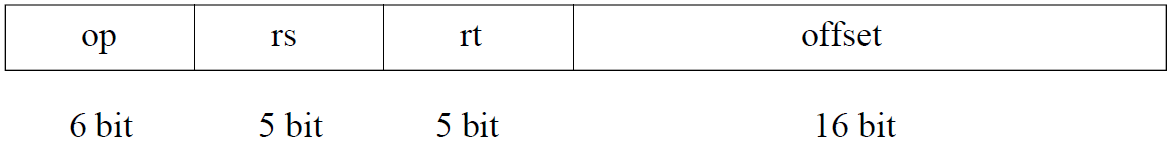
\includegraphics[scale=0.4]{img/loadstore.png}
\caption{Struttura di un'istruzione tipo load/store}\label{fig:loadstore}
\end{figure}
La suddivisione del registro è la seguente:
\begin{description}
\item[op] identifica l'istruzione di tipo load o store
\item[rs] identifica il registro base
\item[rt] identifica il registro sorgente o destinazione per i dati delle operazioni di store o di load da o per la memoria
\item[offset] da sommare all'indirizzo contenuto in \emph{rs} per calcolare l'indirizzo di memoria
\end{description}
\paragraph{Istruzioni di salto}
Per quanto riguarda le istruzioni di salto possiamo suddividerle in due categorie, i salti \emph{condizionati}, che richiedono la verifica di una determinata condizione per decidere se effettuare un salto; oppure istruzioni di salto \emph{incondizionato} che effettuano il salto sempre. 
Lo pseudo assembly di un'istruzione di salto condizionato è:
\begin{verbatim}
beq $s1, $s2, L1	#go to L1 if ($s1 == $s2)
bne $s1, $s2, L1	#go to L1 if ($s1 != $s2)
\end{verbatim}
Le istruzioni di salto condizionato sono nel formato \emph{I-Format}. La suddivisione del registro per questo tipo  di istruzione è mostrata in \figurename\,\ref{fig:condbranch}\\
\begin{figure}[htb]
\centering
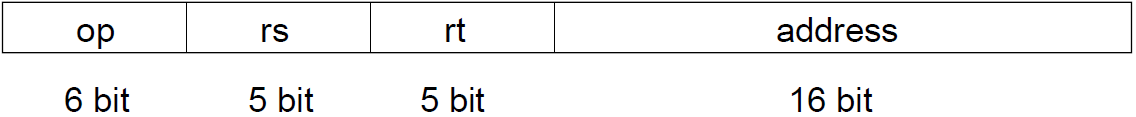
\includegraphics[scale=0.4]{img/condbranch.png}
\caption{Struttura di un'istruzione tipo branch condizionato}\label{fig:condbranch}
\end{figure}
\begin{description}
\item[op] identifica l'istruzione di tipo branch condizionale
\item[rs] identifica il primo registro da comparare
\item[rd] identifica il secondo registro da comparare
\item[address] identifica l'offsett rispetto al PC che corrisponde all'indirizzo dell'etichetta
\end{description}
Per quanto riguarda il salto incondizionato il funzionamento è molto più semplice, quando si raggiunge l'istruzione di salto il PC punta direttamente all'istruzione indicata dall'etichetta. Tale semplicità si rispecchia nella struttura dell'istruzione che in questo caso è di tipo \emph{J-Format}. 
Lo pseudocodice assembly dell'istruzione di salto è:
\begin{verbatim}
j	L1		#go to L1
jr	$s1		#go to add. contenuto in $1
\end{verbatim}
Un esempio di struttura di istruzione di salto è rappresentato in \figurename\,\ref{fig:uncondbranch} 
\begin{figure}[htb]
\centering
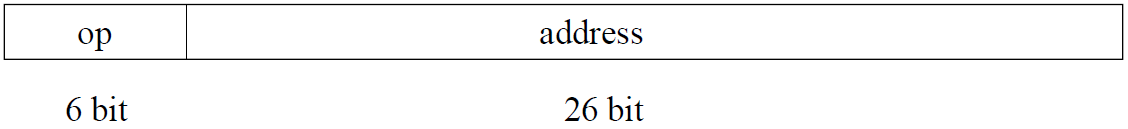
\includegraphics[scale=0.4]{img/uncondbranch.png}
\caption{Divisione delle informazioni in un registro di un istruzione tipo branch incondizionato}\label{fig:uncondbranch}
\end{figure}
dove i valori indicano rispettivamente
\begin{description}
\item[op] identifica il tipo di istruzione
\item[address] identifica l'indirizzo della prossima istruzione da eseguire
\end{description}
Ricapitolando possiamo suddividere le istruzioni in tre categorie in base alla loro struttura e a come vengono eseguite:
\begin{itemize}
\item Tipo R (\emph{Registro})
\begin{itemize}
\item Istruzione ALU
\end{itemize}
\item Tipo I (\emph{Immediate})
\begin{itemize}
\item ALU immediate
\item Istruzioni Load/Store
\item Istruzioni di salto condizionato
\end{itemize}
\item Tipo J (\emph{Jump})
\begin{itemize}
\item Istruzioni di salto incondizionato
\end{itemize}
\end{itemize}
Il perché di questa divisione lo si capisce molto facilmente dallo schema in \figurename\,\ref{fig:rij} nel quale vengono confrontati le diverse suddivisioni degli Instruction Register.
\begin{figure}[htb]
\centering
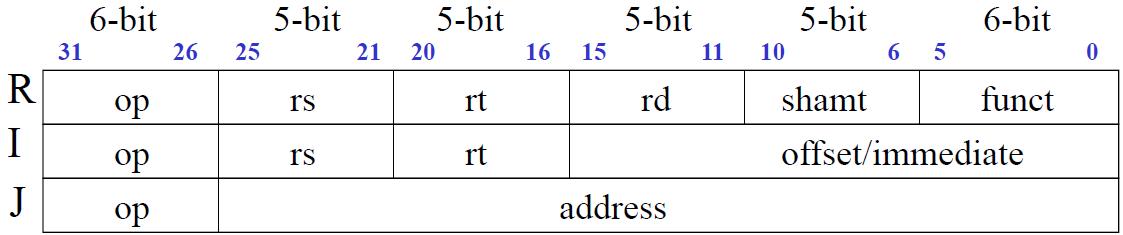
\includegraphics[scale=0.5]{img/rij.png}
\caption{Divisione dei registri nei diversi casi di operazione}\label{fig:rij}
\end{figure}
\subsubsection{Esecuzione delle istruzioni}
Vediamo ora come possono essere implementate le diverse istruzione in ambiente MIPS. Tutte le istruzioni possono essere implementate suddividendo l'esecuzione in cinque fasi distinte:
\begin{enumerate}
\item \textbf{Instruction Fetch Cycle:} durante questo ciclo viene inviato il contenuto del \emph{Program Counter} all'\emph{Instruction Memory} e viene prelevata l'istruzione corrispondente. Successivamente viene aggiornato il PC perchè punti alla prossima istruzione aggiungendo 4 al valore attuale (le istruzioni sono di 4 bytes)
\item \textbf{Instruction Decode and Register Read Cycle:} in questo ciclo si decodifica l'istruzione corrente e si leggono dal \emph{Register File} i registri necessari corrispondenti ai registri specificati nei campi dell'istruzione. Si fa inoltre l'estensione del segno nel caso sia necessario.
\item \textbf{Execution Cycle:} In questo ciclo la ALU effettua le operazioni sugli elementi che sono stati preparati nel ciclo precedente. In base alle istruzioni la ALU esegue le seguenti operazioni
\begin{itemize}
\item Istruzione ALU registro-registro: la ALU esegue le operazioni sugli operandi che ha letto dal \emph{Register File}
\item Istruzioni ALU immediate: la ALU esegue l'operazione specificate sul primo operando letto dal \emph{Register File} e sul operando immediato al quale è stata applicata l'estensione di segno.
\item Istruzioni Load/Store la ALU aggiunge all'indirizzo base l'offset per calcolare l'indirizzo effettivo.
\item Istruzioni di salto condizionato: la ALU compara i due registri e calcola l'indirizzo target del salto da aggiungere al PC
\end{itemize}
\item \textbf{Memory Access (ME):} durante questo ciclo le istruzioni di \emph{Load} effettuano la lettura dalla memoria usando l'indirizzo effettivo calcolato al ciclo precedente, le istruzione di \emph{Store} scrivono nella memoria i dati provenienti dal registro, infine, le istruzioni di \emph{Branch}  aggiornano il valore del Program Counter con l'indirizzo target calcolato al passo precedente, nel caso in cui la condizione sia verificata.
\item \textbf{Write-Back Cycle (WB):} in questo ciclo le istruzioni di \emph{Load} scrivono i dati letti dalla memoria nel registro di destinazione mentre le istruzioni di \emph{ALU} scrivono il risultato delle operazioni nei registri di destinazione.
\end{enumerate}
Come possiamo notare le diverse operazioni non usano sempre tutti i cicli appena descritti ma solitamente (tranne nel caso della \emph{load}) attraversano solo alcune fasi come possiamo vedere dallo schema in \figurename\,\ref{fig:cicli}.\\
Mentre nella tabella di \figurename\,\ref{fig:latency} possiamo vedere le latenze di ogni operazione nel caso di tempo di ciclo uguale ad 1 \emph{ns}.
\begin{figure}[htb]
\centering
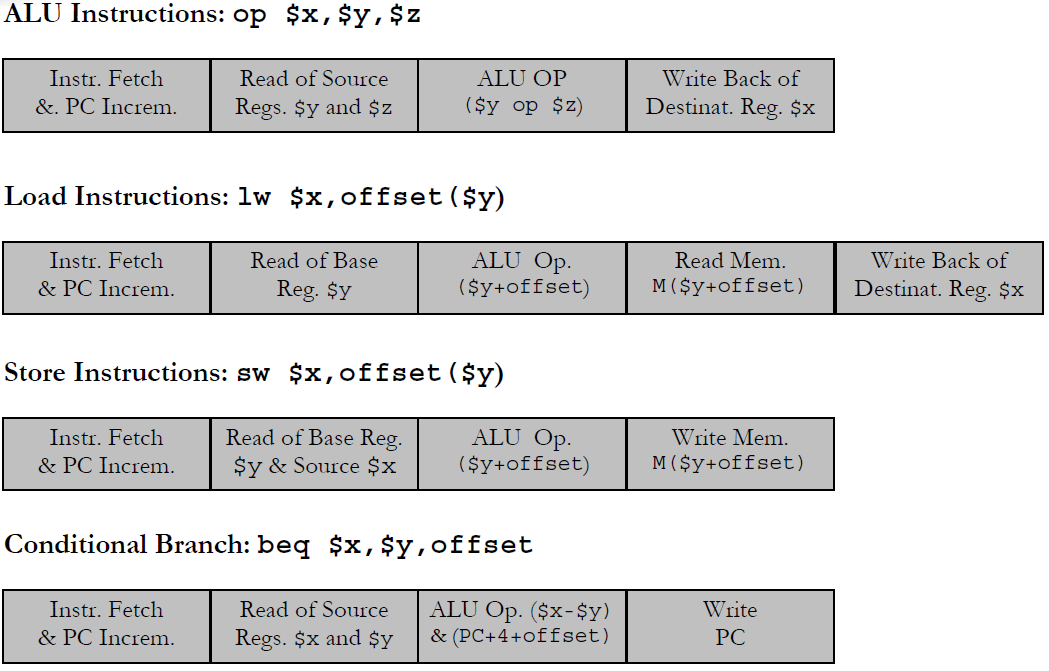
\includegraphics[scale=0.5]{img/cicli.png}
\caption{Cicli eseguiti da ogni operazione}\label{fig:cicli}
\end{figure}
\begin{figure}[htb]
\centering
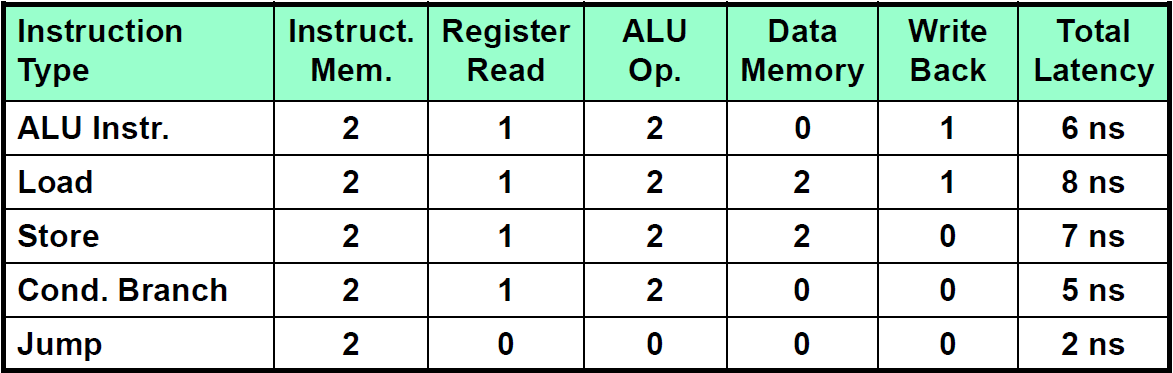
\includegraphics[scale=0.4]{img/latency.png}
\caption{Latenza delle diverse operazioni}\label{fig:latency}
\end{figure}
\subsubsection{Implementazione base di un MIPS}
Vediamo ora come potrebbe essere una semplice implementazione di un \emph{Data Path} in un MIPS. Come notiamo dalla \figurename\,\ref{fig:mips} abbiamo che la parte di memoria dedicata alle istruzioni (\emph{Instruction Memory}) è di sola lettura ed è separata dalla memoria dedicata ai dati (\emph{Data Memory}). Inoltre abbiamo 32 registri organizzati in un \emph{Register File} (RF) con 2 porte di lettura (le due frecce che esco sulla destra) e una porta in scrittura (la freccia in ingresso che punta al campo \emph{Data}).
\begin{figure}[htb]
\centering
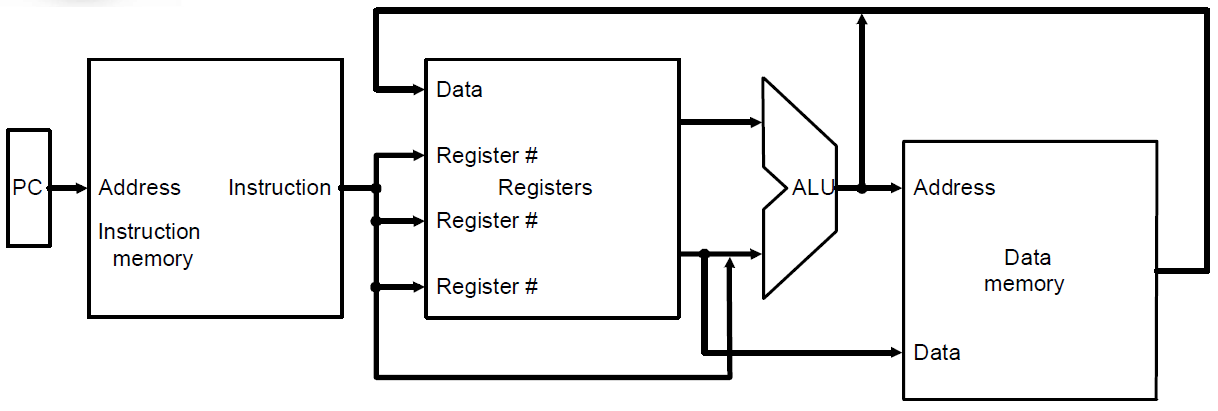
\includegraphics[scale=0.48]{img/mips.png}
\caption{Esempio di implementazione di MIPS}\label{fig:mips}
\end{figure}
La fase di \emph{Instruction Fetch} invece richiede un adder il quale in uscita si connette al PC mentre come ingressi riceve un valore costante \emph{4} mentre all'altro ingresso riceve il valore corrente di del PC come possiamo vedere in \figurename\,\ref{fig:ifetch}.
\begin{figure}[htb]
\centering
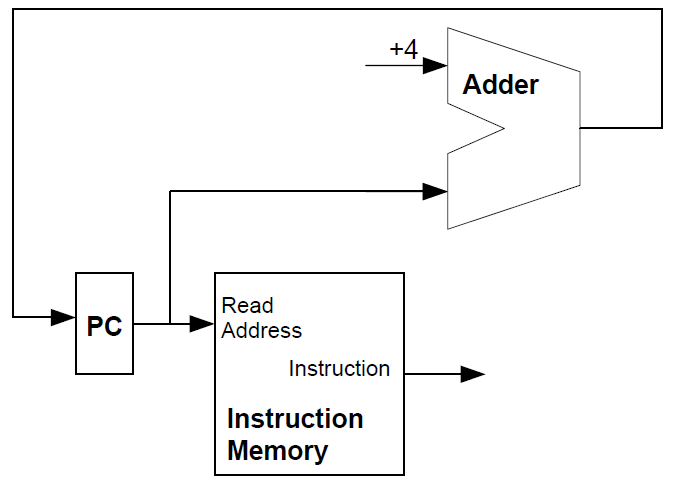
\includegraphics[scale=0.35]{img/ifetch.png}
\caption{Hardware necessario per realizzare l'Instruction Fetch}\label{fig:ifetch}
\end{figure}
Analizziamo ora in breve quale hardware è necessario per implementare le diverse operazioni che possono essere eseguite da un MIPS. Partiamo con l'analizzare un istruzione di tipo ALU come vediamo in \figurename\,\ref{fig:ALUhw}. Dal \emph{Register File} escono due porte che sono connesse ad un'unità ALU la quale ha un uscita \emph{Result} che si connette alla porta di scrittura del \emph{RF} e un'uscita \emph{Zero} per indicare eventuali anomalie. Inoltre la ALU ha un ingresso \emph{OP} che serve a selezionare il tipo di operazione.
\begin{figure}[htb]
\centering
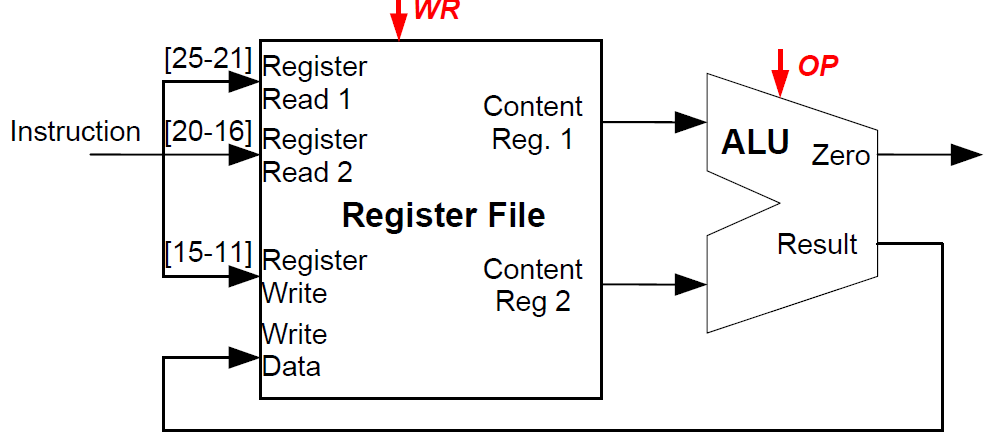
\includegraphics[scale=0.4]{img/aluhw.png}
\caption{Hardware che implementa un istruzione di tipo aritmetico}\label{fig:ALUhw}
\end{figure}
Per quanto riguarda l'istruzione di \emph{load} e quella di \emph{store} sono molto simili come si può vedere da \figurename\,\ref{fig:loadhw} e da \figurename\,\ref{fig:storehw}. Nel caso della load la alu calcola l'indirizzo di memoria da leggere il quale viene inviato alla memoria e il risultato della lettura è registrato tramite la porta write data del \emph{RF}. Nel caso della \emph{store} invece la ALU calcola l'indirizzo di destinazione della scrittura e tramite la porta write del \emph{Data Memory} viene copiato il valore del registro.
\begin{figure}[htb]
\centering
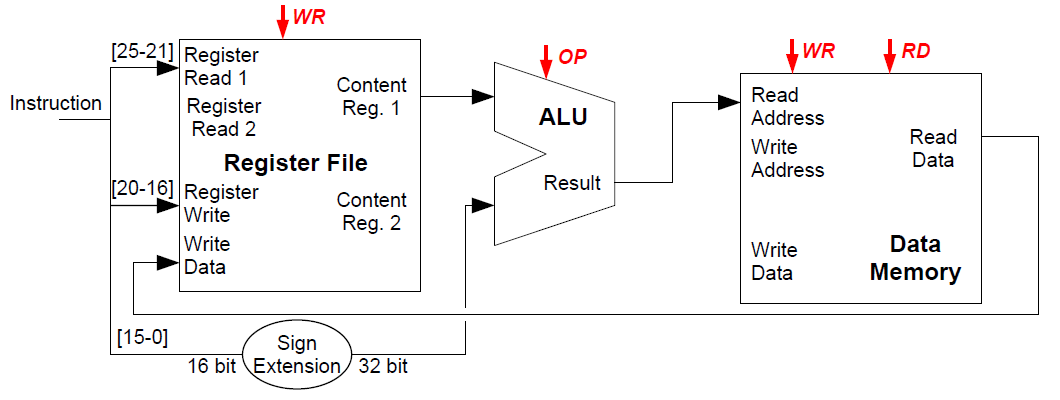
\includegraphics[scale=0.45]{img/loadhw.png}
\caption{Hardware che implementa un istruzione di tipo load}\label{fig:loadhw}
\end{figure}
\begin{figure}[htb]
\centering
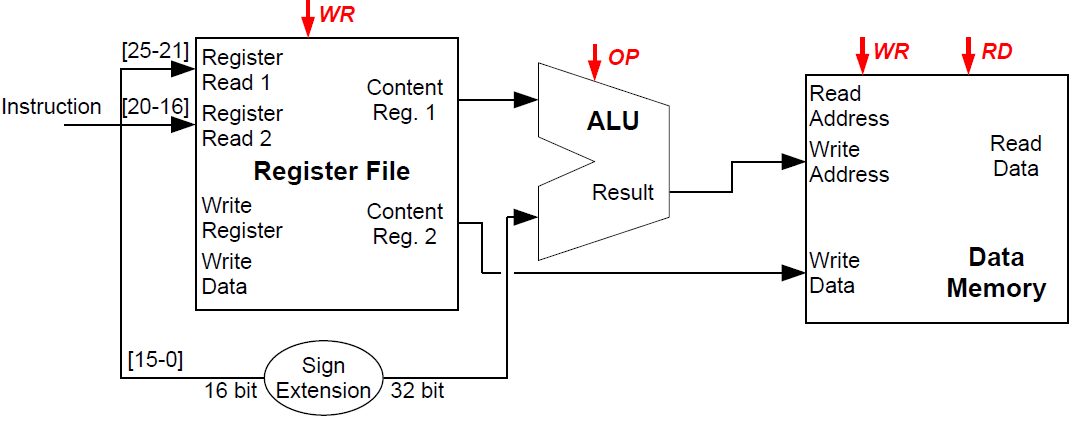
\includegraphics[scale=0.45]{img/storehw.png}
\caption{Hardware che implementa un istruzione di tipo store}\label{fig:storehw}
\end{figure}
In entrambi i casi un unità particolare si occupa di eseguire l'estensione del segno in caso di bisogno.\\
Stabiliamo ora come viene implementato il clock del circuito; possiamo avere due possibilità, la prima è avere un unico ciclo di clock lungo quanto il percorso critico necessario per eseguire l'istruzione di load (la più lunga), la seconda è avere un ciclo di clock lungo quanto un singolo passaggio in uno dei componenti prima analizzati.\\
Analizziamo innanzitutto il caso di singolo ciclo, in questo caso il ciclo dovrà avere una durata pari al tempo necessario per eseguire un'istruzione di load che come abbiamo visto è pari a $T = 8 ns \quad (f=125 \ MHz)$. Assumiamo quindi che ogni istruzione verrà eseguita in un singolo ciclo di clock, ogni modulo verrà utilizzato una sola volta per clock e quei moduli che dovrebbero essere utilizzati più di una volta dovranno essere duplicati.
Inoltre dobbiamo tener conto anche delle differenze tra i diversi tipi di istruzioni, infatti, all'ingresso di scrittura dell'RF possiamo avere dati provenienti da una ALU e quindi di lunghezza [15-11] bit oppure dati provenienti da una load/store con una lunghezza di [20-16] bit questo richiede un \emph{Multiplexer} all'ingresso dei registri nel RF. In secondo luogo al secondo ingresso della ALU possiamo avere avere il dato proveniente da un registro nel caso di operazioni ALU oppure l'offset per le istruzioni di load/store, questo richiede un \emph{MUX} al secondo ingresso della ALU. Infine i dati all'output del Destination Register possono arrivare sia dal risultato della ALU oppure dal Data Memory nel caso di load questo comporta l'utilizzo di un \emph{MUX} all'ingresso in scrittura dei dati su RF.
In \figurename~\ref{fig:monocic} vediamo l'implementazione completa di un MIPS a ciclo singolo con l'introduzione, oltre che dei MUX precedentemente specificati, anche di una ALU (parte alta della figura) che permette l'implementazione dei branch, e della logica di controllo (in rosso nella figura)\\
Veniamo ora al caso in cui il ciclo di clock sia di lunghezza pari al tempo necessario per un singolo modulo $T = 2 ns$ questo significa che per eseguire un'istruzione di load sono necessari 5 cicli di clock per un totale di \emph{10ns}. Ogni fase dell'istruzione richiede un ciclo di clock ma questo permette la condivisione dei moduli tra diverse istruzioni in differenti cicli di clock, anche se questo richiede l'inserimento di registri tra un'unità  e l'altra.
\begin{figure}[!Hptb]
\centering
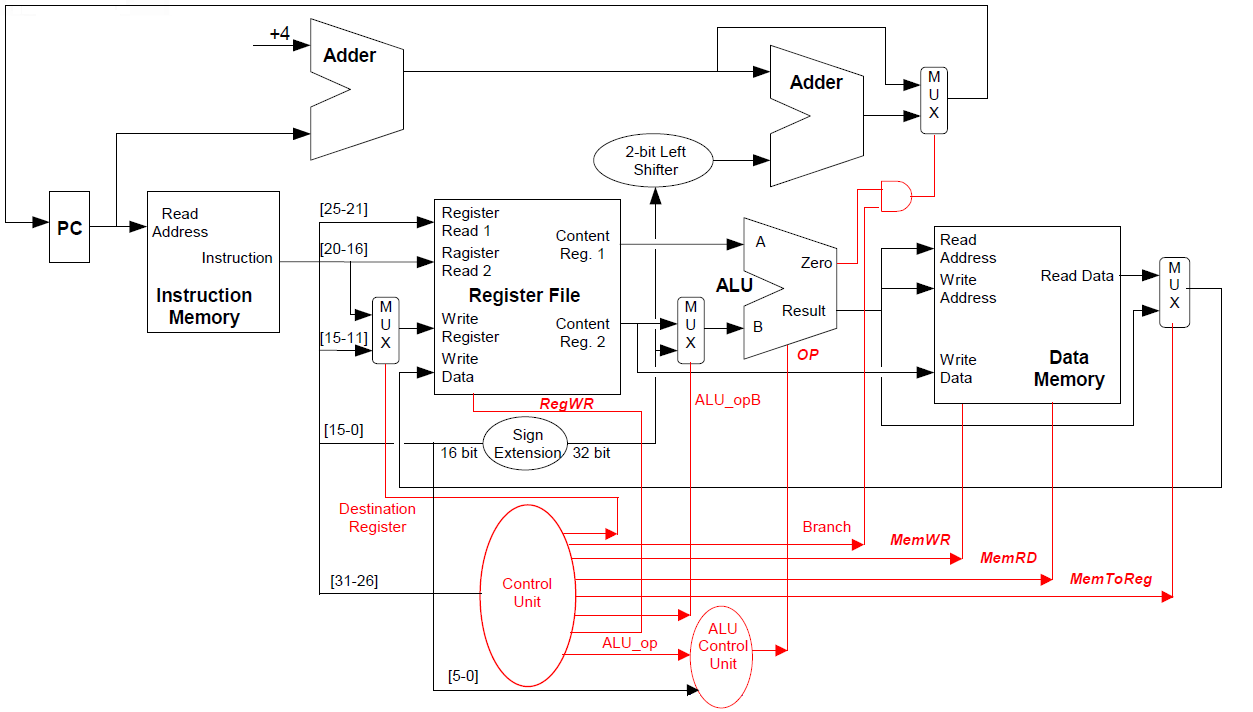
\includegraphics[scale=0.67, angle=90]{img/monocic.png}
\caption{MIPS a singolo ciclo con logica di controllo}\label{fig:monocic}
\end{figure}
\subsection{Pipelining}
Il pipelining è una tecnica di ottimizzazione basata sull'esecuzione multipla sovrapposta di istruzioni sequenziali. L'idea fondamentale è quella di sfruttare il parallelismo intrinseco delle istruzioni sequenziali in quanto l'esecuzione di una istruzione è suddivisa in fasi differenti (\emph{pipelines stages}) che richiedono soltanto una piccola frazione di tempo per essere completate. I diversi stati sono connessi in sequenza nella pipeline, un'istruzione entra da una parte procede attraverso i diversi stadi e esce all'altro capo come in una catena di montaggio.\\
I vantaggi di questa tecnica è che è completamente trasparente al programmatore, inoltre come in una catena di montaggio, il tempo necessario per eseguire un'istruzione è uguale al caso in cui l'istruzione sia eseguita senza pipeline; quello che la pipeline fa è incrementare il numero di istruzioni eseguite contemporaneamente e perciò aumentare la frequenza di completamento come vediamo in \figurename\,\ref{fig:seqvspipe}\\
\begin{figure}[tb]
\centering
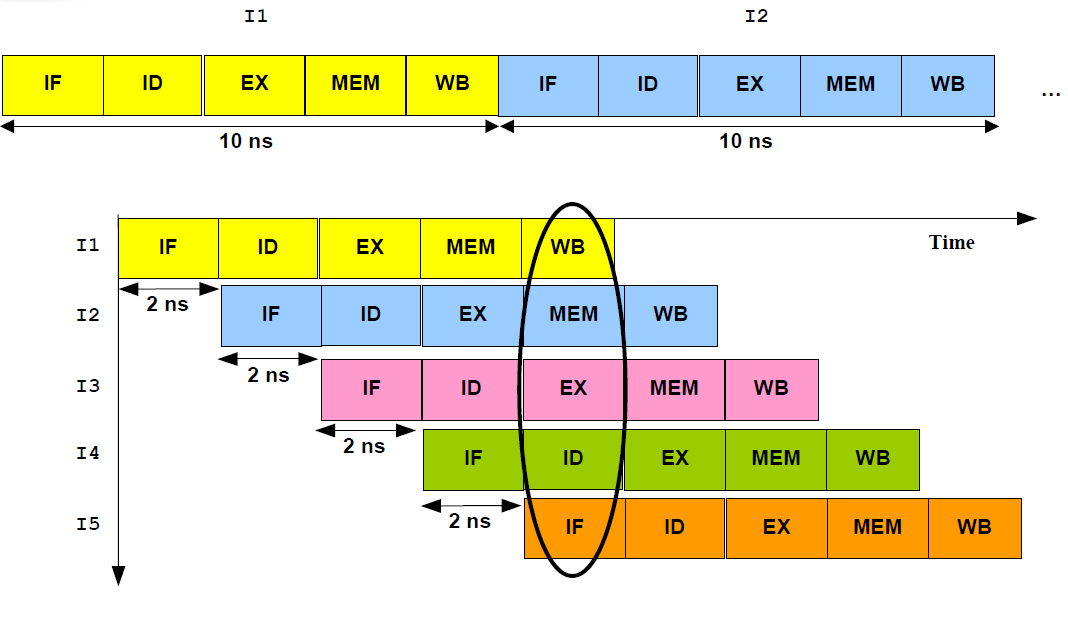
\includegraphics[scale=0.4]{img/seqvspipe.png}
\caption{Confronto tra esecuzione sequenziale e pipelined}\label{fig:seqvspipe}
\end{figure}
Il tempo necessario per far avanzare un'istruzione di una fase corrisponde ad un ciclo di clock, le diverse fasi perciò devono essere \emph{sincronizzate}, il periodo di clock deve essere uguale al tempo di esecuzione della fase più lenta (nel nostro esempio 2ns). L'obiettivo è quello di bilanciare la lunghezza di ogni fase della pipeline in modo da avere uno \emph{speedup ideale} uguale al numero di fasi della pipeline.\\
Nel caso ideale vediamo come la pipeline sia più efficiente sia dell'architettura a singolo ciclo che a quella multi-ciclo viste in precedenza.
Nel caso di una CPU1 non pipeline con un unico ciclo di clock della durata di 8ns contro una CPU2 con una pipeline a 5 stadi e ciclo di 2ns abbiamo che:
\begin{itemize}
\item la \emph{latenza} ovvero il tempo necessario per eseguire una istruzione è peggiore nel caso di CPU2: 8ns vs 10ns
\item il \emph{throughput} tuttavia è notevolmente migliorato: $1 \ istruzione/8ns$ vs $1 \ istruzione/2ns$
\end{itemize}
Nel caso di CPU3 multi-ciclo senza pipeline contro un'architettura CPU2 come quella descritta in precedenza abbiamo:
\begin{itemize}
\item la \emph{latenza} resta invariata: 10 ns
\item il \emph{throughput} cresce di ben 5 volte: $1 \ istruzione/10ns$ vs $1 \ istruzione/2ns$
\end{itemize}
\subsubsection{Implementazione di una Pipeline}
Innanzitutto vediamo quali fasi devono attraversare ciascuna operazione in quanto non tutte le fasi sono necessarie per tutte le operazioni, uno schema riassuntivo è specificato in \figurename\,\ref{fig:pipefasi}.\\
\begin{figure}[tbh]
\centering
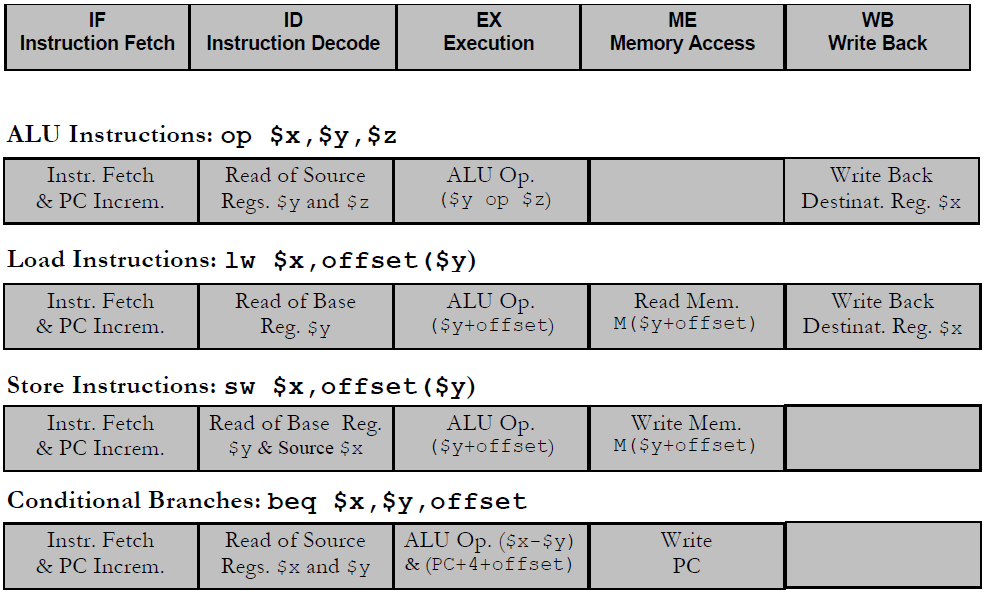
\includegraphics[scale=0.4]{img/pipefasi.png}
\caption{Fasi della pipeline necessarie ad ogni istruzione}\label{fig:pipefasi}
\end{figure}
La divisione dell'esecuzione di una istruzione in 5 fasi implica che in ogni ciclo di clock cinque istruzione sono in esecuzione questo comporta la necessità di inserire dei \emph{registri} tra una fase e l'altra della pipeline per separare i diversi stage.\\
In \figurename\,\ref{fig:pipeline} vediamo una possibile implementazione di un'architettura MIPS pipelined con l'introduzione dei registri tra le fasi (in verde).
\begin{figure}[!Hptb]
\centering
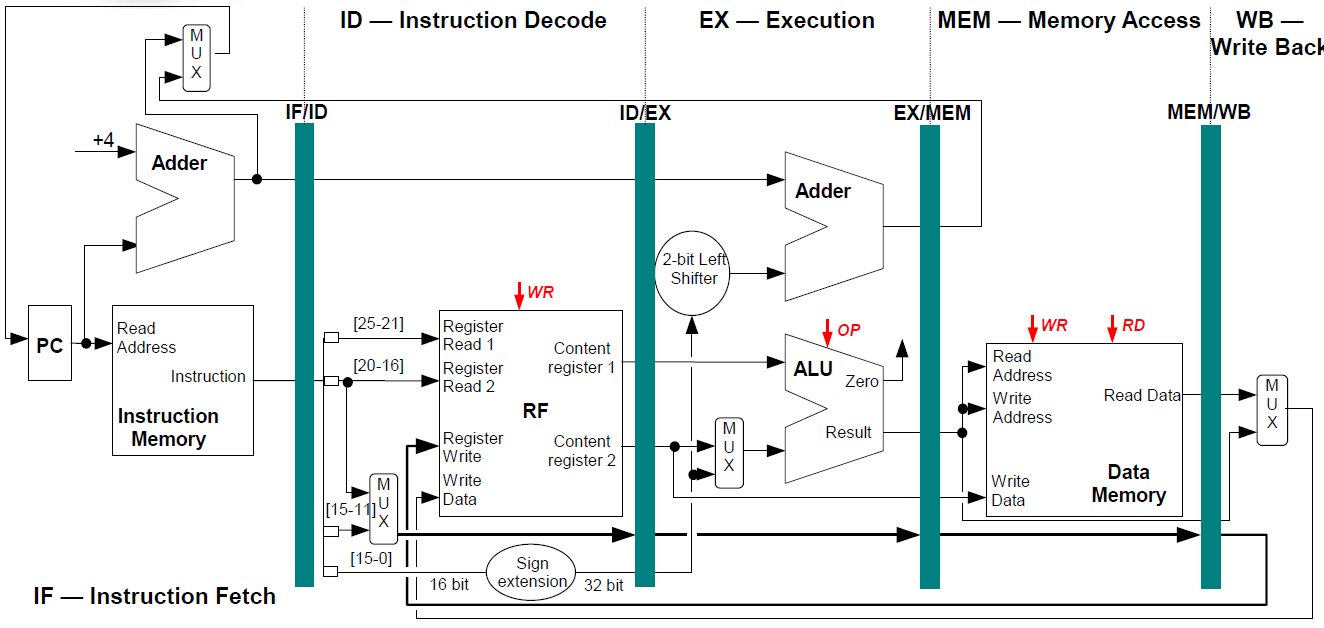
\includegraphics[scale=0.6, angle=90]{img/pipeline.png}
\caption{Schema di un MIPS con pipeline}\label{fig:pipeline}
\end{figure}
\pagebreak
\subsection{Il problema del ''Hazard''}
Si ha un \emph{hazard} quando vi è una dipendenza tra istruzioni diverse e la sovrapposizione dovuta al pipeline cambia l'ordine di dipendenza sugli operandi. Hazard previene l'esecuzione della prossima istruzione nel ciclo di clock designato ma così facendo riduce le performance allontanandole dallo speedup ideale.\\
Possiamo distinguere tre classi di \emph{hazard}:
\begin{itemize}
\item \textbf{Structural Hazards:} si ha quando diverse istruzioni cercano di utilizzare la stessa risorsa simultaneamente (stessa memoria per istruzioni e dati)
\item \textbf{Data Hazards:} si ha quando si cerca di utilizzare un risultato prima che questo sia pronto(istruzione dipendente dalla precedente che è nella pipeline)
\item \textbf{Control Hazards:} si ha quando si deve prendere una decisione sulla esecuzione della prossima istruzione prima della valutazione di una condizione (branch condizionali)
\end{itemize}
Tra questi tre tipi di hazard il primo non può presentarsi nelle architetture MIPS in quanto lo spazio di memoria dedicato alle istruzioni e quello dedicato ai dati sono fisicamente separati.
\subsubsection{Data Hazard}
Per quanto riguarda il data hazard si verifica quando sono in esecuzione nella pipeline due o più istruzioni \emph{dipendenti}.
\begin{verbatim}
sub   $2, $1, $3
and   $12, $2, $5   #1° operando dipende dalla sub
or    $13, $6, $2   #2° operando dipende dalla sub
add   $14, $2, $2   #1° & 2° operando dipendono dalla sub
sw    $15, 100($2)  #Il registro base dipende dalla sub
\end{verbatim}
Come vediamo dall'esempio qui sopra e dalla sua esecuzione in \figurename\,\ref{fig:datahazard} abbiamo che le istruzioni successive alla \texttt{sub} debbono aspettare che la prima istruzione arrivi nella fase di \emph{write-back} prima di poter utilizzare il dato come avviene per l'ultima istruzione evidenziata da una freccia verde.
\begin{figure}[htb]
\centering
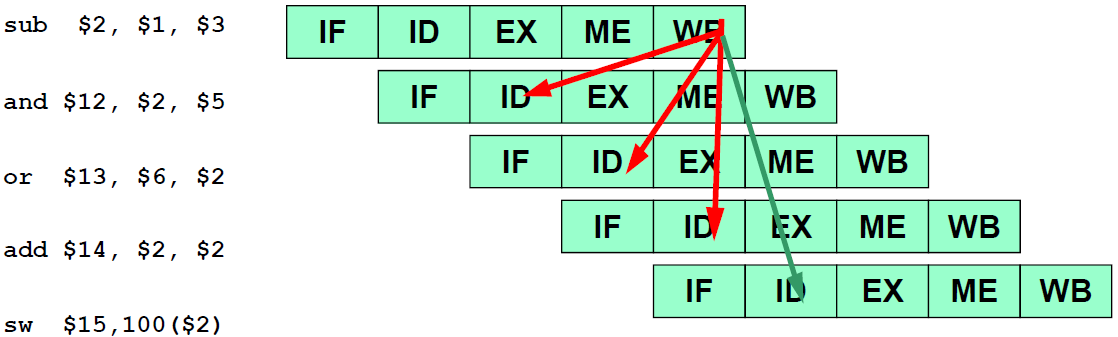
\includegraphics[scale=0.5]{img/datahazard.png}
\caption{Esempio di data hazard}\label{fig:datahazard}
\end{figure}
Esistono diversi meccanismi per far si che queste dipendenze vengano soddisfatte, le principali si possono suddividere in due categorie:
\begin{itemize}
\item \textbf{Tecniche di compilazione:} in questa categoria rientra il re-scheduling delle operazioni che connsiste nell'inserire istruzioni indipendenti tra le istruzioni correlate in modo da permettere il calcolo dei valori necessari; nel caso non sia possibile inserire altre operazioni il compilatore inserisce delle \texttt{nop} ovvero delle operazioni che non fanno nulla \emph{no operation}
\item \textbf{Tecniche hardware:} in questa categoria rientrano la possibilità di inserire delle \emph{bubbles} o degli stalli oppure le tecniche di \emph{Data Forwarding} e di \emph{Bypassing}
\end{itemize}
Vediamo innanzi tutto un esempio di inserimento di \texttt{nop} in \figurename\,\ref{fig:nop}
\begin{figure}[htb]
\centering
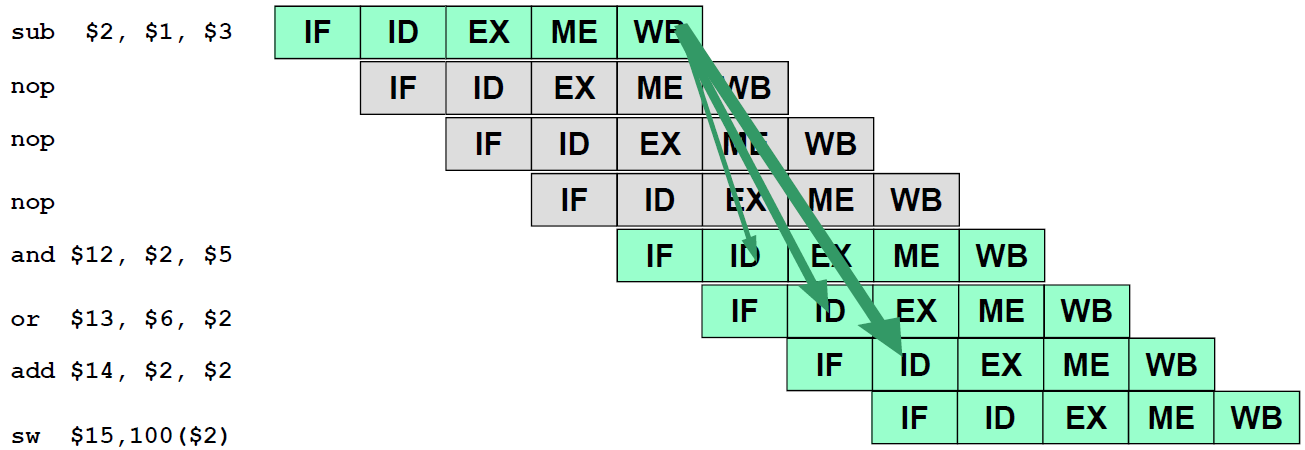
\includegraphics[scale=0.45]{img/nop.png}
\caption{Esempio di uso \texttt{nop}}\label{fig:nop}
\end{figure}
Come vediamo l'inserimento di nop perggiora lo speedup ideale, cosa che invece non succede se si applicano le tecniche di re-scheduling in quanto non vengono inserite istruzioni inutili nell'esecuzione  delle istruzioni ma viene modificato semplicemente l'ordine nel quale vengono eseguite.\\
Il caso di inserimento di stalli è molto simile a quello di inserimento delle nop la differenza sta nel fatto che si ferma l'esecuzione dell'istruzione dipendente il tempo necessario affinché l'istruzione in esecuzione renda disponibile il dato come vediamo in \figurename\,\ref{fig:stall}, anche in questo caso abbiamo un peggioramento dello speedup ideale.
\begin{figure}[htb]
\centering
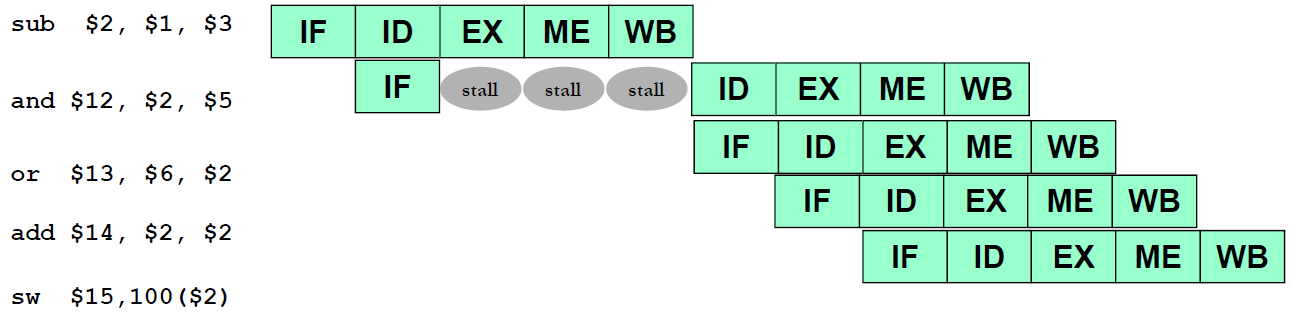
\includegraphics[scale=0.45]{img/stall.png}
\caption{Esempio di uso degli stalli}\label{fig:stall}
\end{figure}
\paragraph{Data Forwarding}
Il \emph{data forwarding} è una tecnica hardware che comporta l'utilizzo dei risultati temporanei immagazzinati nei registri della pipeline, per fare ciò abbiamo bisogno di aggiungere dei \emph{multiplexer} all'ingresso della ALU per selezionare la provenienza dei dati. In \figurename\,\ref{fig:forwardingpath} vediamo quali sono i collegamenti necessari per l'esecuzione di istruzioni aritmetiche dipendenti; questi path sono tre:
\begin{itemize}
\item\textbf{EX/EX path:} in figura da ALU ad ALU che risolve il problema di due istruzioni consecutive nella quale la seconda necessita del risultato della prima. Nell'esempio precedente la dipendenza \texttt{sub}$\rightarrow$\texttt{and}
\item\textbf{MEM/EX path:} in questo caso si risolve la dipendenza tra la prima e la terza istruzione (\texttt{sub}$\rightarrow$\texttt{or})
\item\textbf{MEM/ID path:} risolve la dipendenza tra la prima e la quarta istruzione (\texttt{sub}$\rightarrow$\texttt{add})
\end{itemize}
Con l'introduzione di questi path si riesce a risolvere tutti i problemi di dipendenza per quanto riguarda le istruzioni di tipo aritmetico.
In \figurename\,\ref{fig:forwardingcirc} vediamo una possibile implementazione hardware di una pipeline con sistema di forwarding path.
\begin{figure}[htb]
\centering
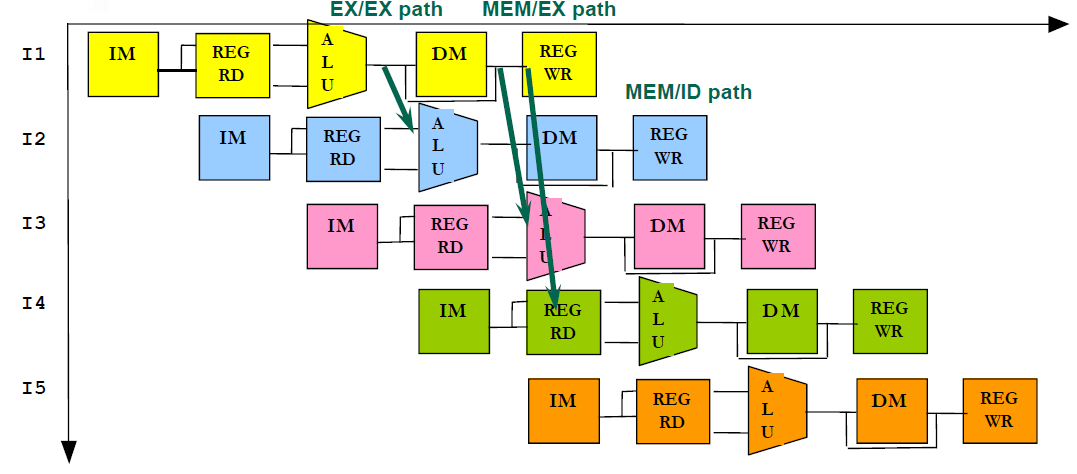
\includegraphics[scale=0.45]{img/forwardingpath.png}
\caption{Esempio di forwarding path}\label{fig:forwardingpath}
\end{figure}
\begin{figure}[htb]
\centering
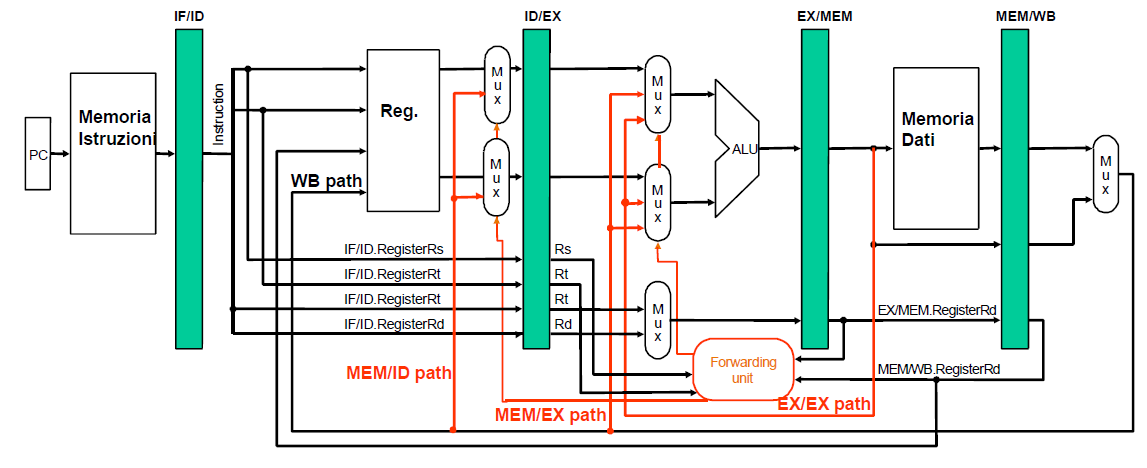
\includegraphics[scale=0.7,angle=90]{img/forwardingcirc.png}
\caption{Schema MIPS con forwarding}\label{fig:forwardingcirc}
\end{figure}
Esiste ancora una situazione però in cui è necessario inserire degli stalli, questa situazione è dovuta alla sequenza di istruzioni seguenti:
\begin{verbatim}
L1: lw  $s0, 4($t1)     #$s0<-M[4 + $t1]
L2: add $s5, $s0, $s1   #1° operand depends from L1
\end{verbatim}
Questa dipendenza si crea in quanto il dato viene scritto in \texttt{\$s0} solo nella fase di WB mentre viene letto durante la fase di ID. In questo caso non si può fare molto se non sfruttare il forwarding path MEM/EX già analizzato prima anche se comunque è necessario introdurre uno stallo per risolvere la dipendenza.
Nel caso invece in cui la dipendenza sia tra un'istruzione di \emph{load} e una di \emph{store} si può risolvere la dipendenza aggiungendo un \emph{forwarding path} tra le due fasi di MEM. Questo path permette di risolvere la dipendenza senza dover introdurre altri stalli come si può vedere in \figurename\,\ref{fig:memmempath}.
\begin{figure}
\centering
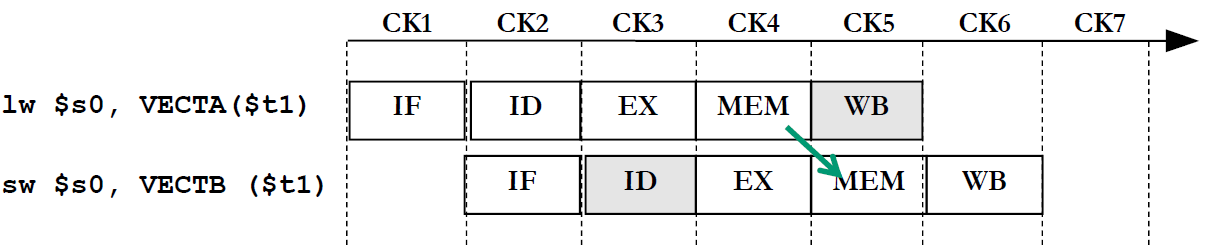
\includegraphics[scale=0.5]{img/memmempath.png}
\caption{Forwarding path tra due fasi di memorizzazione successive.}\label{fig:memmempath}
\end{figure}
Con l'architettura attuale, come abbiamo visto, nel caso di dipendenza tra una \emph{load} ed un'istruzione aritmetica che legge un registro è necessario introdurre uno stallo; in quanto l'accesso in lettura avviene durante la fase di ID mentre la scritture avviene durante la fase di WB. Nel caso, invece, di \emph{pipeline ottimizzata} possiamo assumere che la fase di lettura avviene nelle seconda metà del ciclo di clock mentre la fase di scrittura nella prima metà; in questo modo nel caso in cui lettura e scrittura facciano riferimento allo stesso registro nello stesso ciclo di clock non è più necessario inserire degli stalli, e si può inoltre eliminare il forwarding path tra MEM e ID.
\subsubsection{Altri tipi di Data Hazard}
Fino ad ora abbiamo analizzato solo un tipo di dipendenza sui dati, questo tipo di dipendenza è chiamato \textbf{RAW (Read After Write)}, e si ha quando l'istruzione \emph{n+1} cerca di leggere un registro prima che l'istruzione n abbia finito di scrivere tale registro.\\
Esistono tuttavia altri due tipi di \emph{data hazard} che sono:
\begin{itemize}
\item Write After Write (WAW)
\item Write After Read (WAR)
\end{itemize}
La dipendenza di tipo WAW si ha quando un istruzione n+1 di tenta di scrivere un registro il quale non è ancora stato scritto dall'istruzione n. Tale tipo di dipendenza avviene solo nel caso in cui la nostra pipeline preveda la possibilità di fasi di memorizzazione o di esecuzione multi-ciclo come mostrato in \figurename\,\ref{fig:multimem} e \ref{fig:multiexe} le quali portano alla terminazione delle istruzione fuori ordine
\begin{figure}
\centering
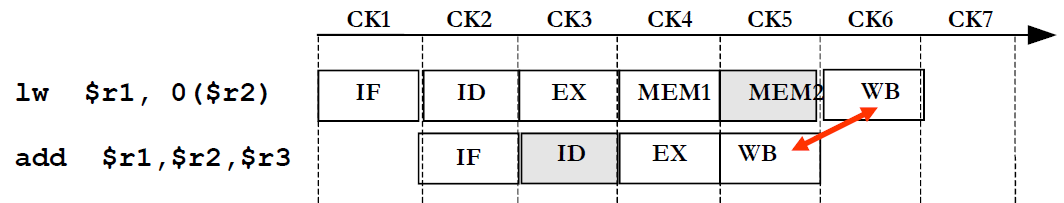
\includegraphics[scale=0.4]{img/multimem.png}
\caption{Fase di memorizzazione multiciclo che porta alla creazione di dipendenze di tipo WAW}\label{fig:multimem}
\end{figure}
\begin{figure}
\centering
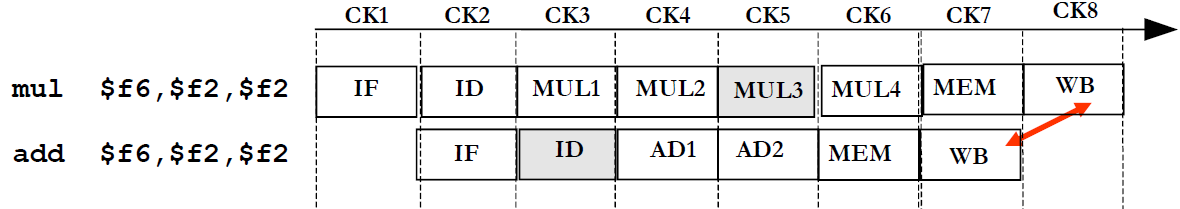
\includegraphics[scale=0.4]{img/multiexe.png}
\caption{Fase di esecuzione multiciclo che porta alla creazione di dipendenze di tipo WAW}\label{fig:multiexe}
\end{figure}
Per quanto riguarda le dipendenze di tipo WAR si hanno quando l'istruzione n+1 tenta di scrivere un registro prima che questo sia stato letto da un istruzione n, nel caso di architettura MIPS però tale tipo di dipendenza non può mai verificarsi in quanto la lettura avviene nella fase ID mentre la scrittura nella fase WB.
\subsection{Analisi delle performance}
L'utilizzo della pipeline aumenta il throughput della CPU ma non riduce il tempo di esecuzione della singola istruzione, anzi solitamente aumenta la latenza di ogni istruzione bisogna quindi bilanciare il numero di fasi con l'overhead dovuto alla pipeline.\\
Definito $IC = Instruction \ Count$ ovvero il numero di istruzioni eseguite, possiamo determinare il numero di cicli di clock necessari per completare queste operazioni operazione. Tale valore è uguale a:
$$\#Clock \ Cycle = IC + \# Stall \ Cycles + 4$$
Dividendo tale valore per il numero di operazioni otteniamo:
$$
\begin{array}{rcl}
CPI & = &Clock \ Per \ Instruction = \# Clock \ Cycle /IC = \\
& = & (IC + \#Stall \ Cycles + 4)/IC
\end{array}
$$
$$MIPS= f_{clock} / (CPI * 10^6)$$
Come visto fino ad ora la CPI ideale per la pipeline è 1 ma gli stalli degradano le performance.
Abbiamo così che la CPI media è data da:
$$
\begin{array}{rcl}
Ave. \ CPI & = & Ideal \ CPI + \#Stall \ per \ Instruction \\
& = & 1 + \#Stall \ per \ Instruction
\end{array}
$$
Possiamo misurare il miglioramento delle performance dato dall'introduzione della pipeline come
$$
\begin{array}{rcl}
Pipeline \ SpeedUp & = & \frac{Ave. \ Exec. \ Time \ Unpipelined}{Ave. \ Exec. \ Time \ Pipelined} = \\
& = & \frac{Ave. \ CPI \ Unp.}{Ave. \ CPI \ Pipe} \times \frac{Clock \ Cycle \ Unp.}{Clock \ Cycle \ Pipe}
\end{array}
$$
Se ignoriamo l'overhead sul tempo di clock e assumiamo che i diversi stage siano perfettamente bilanciati possiamo ridefinire lo speedup come
$$SpeedUp_{pipeline} = \frac{Ave. \ CPI \ Unp.}{1 + \# Stall \ per \ Instruction}$$
Nel caso ideale nel quale tutte le istruzioni richiedano lo stesso numero di cicli questi sono uguali al numero di fasi della pipeline e possiamo riscrivere la precedente come:
$$SpeedUp_{pipeline} = \frac{Pipeline \ Depth}{1 + \# Stall \ per \ Instruction}$$
Nel caso ideale in cui non ci siano stalli vediamo come le performance migliori tanto è più profonda (maggior numero di fasi) la pipeline.\\
Nel caso in cui si abbiano dei salti condizionati le performance peggiorano in base alla penalità del branch, infatti:
$$SpeedUp_{pipeline} = \frac{Pipeline \ Depth}{1 + Branch \ Frequency \times Branch \ Penalty}$$


%\section{Tecniche di predizione dei salti}\label{capitolo2}
Come abbiamo visto nel \chaptername\,\ref{capitolo1} i branch condizionati sono istruzioni di salto che vengono eseguite soltanto se viene soddisfatta la condizione. L'indirizzo di destinazione del branch viene sostituito nel program counter al posto dell'indirizzo dell'istruzione sequenziale successiva.
Nel caso di ambiente MIPS possiamo distinguere due tipi di branch:
\begin{itemize}
\item \texttt{beq}: \emph{branch on equal} che richiede che i valori nei registri da confrontare siano uguali.
\item \texttt{bne}: \emph{branch on not equal} che richiede che i valori nei registri da confrontare siano diversi.
\end{itemize}
Come abbiamo visto nel capitolo precedente le istruzioni di salto condizionato sono nel formato \emph{I-Format} e un'istruzione di questo tipo è suddivisa nei diversi campi come mostrato in \figurename\,\ref{fig:branch}
\begin{figure}
\centering
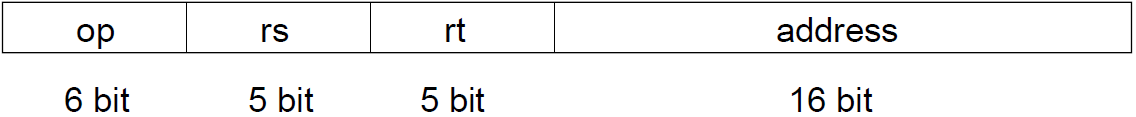
\includegraphics[scale=0.5]{img/condbranch.png}
\caption{Esempio di istruzione di branch}\label{fig:branch}
\end{figure}
Dove il campo \texttt{address} indica l'indirizzo relativo rispetto al program counter che punta all'etichetta di salto.\\
Questo tipo di istruzione sfrutta solo quattro dei cinque stadi della pipeline come mostrato in \figurename\,\ref{fig:branchpipe}; durante l'instruction fetch si recupera l'istruzione da eseguire e si aggiorna il program counter all'istruzione sequenziale successiva, successivamente durante la fase di instruction decode si leggono i due registri da comparare. Durante la fase di \emph{execution} la ALU compara i due registri e calcola il valore di destinazione del salto. Durante la fase \emph{Memory Access} si decide in base al valore della comparazione effettuata dalla ALU se aggiornare il PC con il valore del salto.
\begin{figure}
\centering
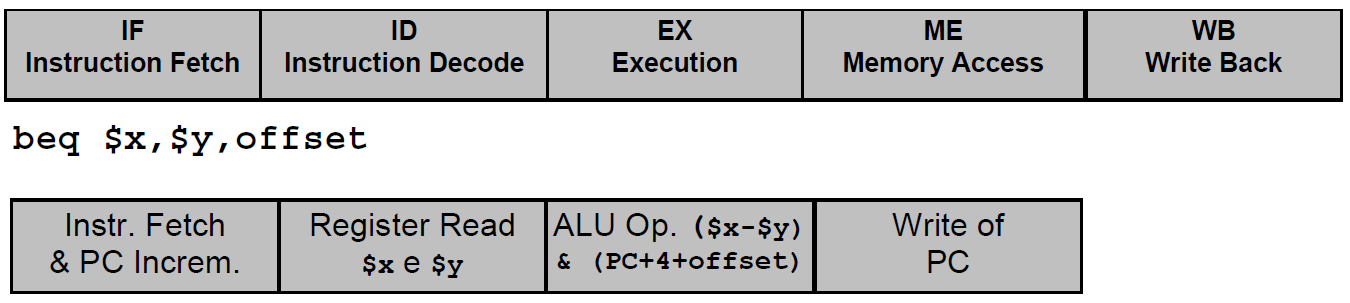
\includegraphics[scale=0.5]{img/branchpipe.png}
\caption{Suddivisione dell'esecuzione di un'istruzione di salto nelle varie fasi di una pipe}\label{fig:branchpipe}
\end{figure}
\subsection{Il problema del Control Hazard}
Il \emph{control hazard} è il problema di decidere quale istruzione eseguire prima che la condizione di salto sia valutata. I problemi di \emph{control hazard} nascono ogni qualvolta nella pipeline sia necessario modificare il valore del PC. Tali problemi riducono percio la velocità della pipeline riducendo lo speedup ideale a causa di introduzioni di stalli nella pipeline.\\
Per alimentare la pipeline è necessario prelevare una nuova istruzione ad ogni ciclo di clock ma la decisione se effettuare o non effettuare un salto avviene solo durante lo stage \emph{MEM}. Questo ritardo nel determinare l'istruzione successiva corretta è chiamato \emph{Control Hazard} o \emph{Conditional Branch Hazard}.\\
Analizziamo ora l'esempio di \figurename\,\ref{fig:branchexe} in questo esempio la prima istruzione è un salto condizionato che viene valutato solo nella fase si MEM; durante l'esecuzione di tale istruzione vengono prelevate anche le tre istruzioni successive per continuare ad alimentare la pipeline. Se il salto non viene eseguito l'esecuzione è corretta e può proseguire, nel caso in cui, invece, il salto venga eseguito allora diventa necessario effettuare il \emph{flush} delle tre istruzioni prelevate durante l'esecuzione del branch.
\begin{figure}
\centering
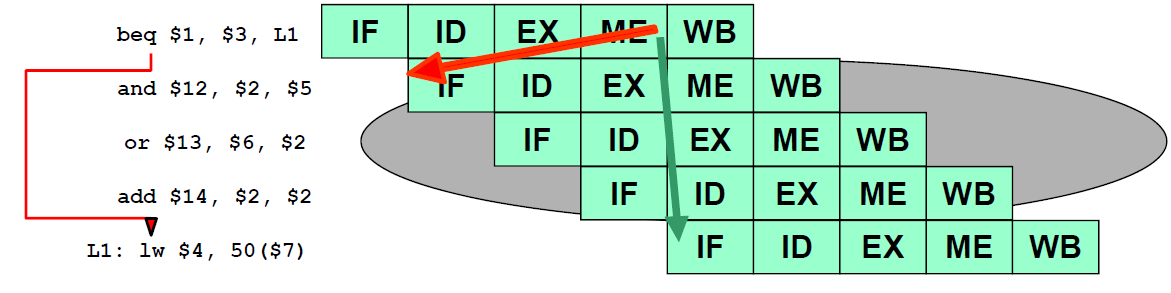
\includegraphics[scale=0.5]{img/branchexe.png}
\caption{Esempio di esecuzione di un istruzione di salto}\label{fig:branchexe}
\end{figure}
Una possibile soluzione al problema è quella di attendere la decisione del salto prima di effettuare qualsiasi altra operazione; questo comporta l'inserimento di "stalli" nella pipeline; più precisamente sono necessari:
\begin{itemize}
\item tre stalli senza forwarding
\item due stalli con forwarding
\end{itemize}
Nel caso in cui il salto non venga eseguito, tuttavia, la penalità di tre cicli   di stallo non è giustificata. Un'altra soluzione è quella di assumere che il salto non sia mai eseguito e quindi scartare le tre istruzioni nel caso in cui il salto venga preso.\\
Una terza soluzione è quella di aggiungere delle risorse hardware per permettere di:
\begin{itemize}
\item comparare i registri
\item calcolare l'indirizzo di destinazione del branch
\item aggiornare il valore del PC
\end{itemize}
il prima possibile nella catena della pipeline.
Nei processori MIPS tutto questo avviene durante lo stage ID come mostrato in \figurename\,\ref{fig:hwbranch}
\begin{figure}
\centering
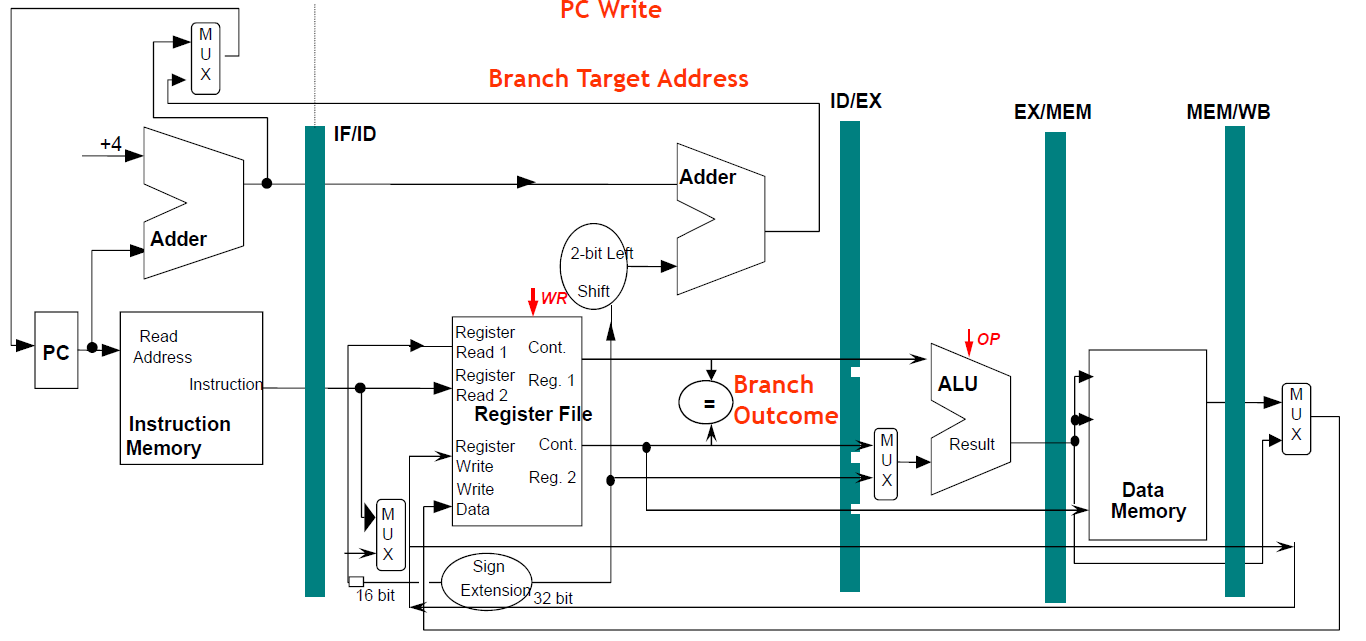
\includegraphics[scale=0.4,angle=90]{img/hwbranch.png}
\caption{Hardware aggiuntivo per risolvere i problemi di controllo}\label{fig:hwbranch}
\end{figure}
Utilizzando queste tecniche si riesce a ridurre al minimo il costo per recuperare la corretta esecuzione di un branch nel caso di scelta sbagliata, riducendo a uno il numero degli stalli da introdurre.\\
Tuttavia queste tecniche comportano tuttavia una riduzione delle performance quantificabile tra il $10\%$ e il $30\%$ in base alla frequenza dei salti.
Tali perdite di performance possono essere ridotte ulteriormente tramite alcune tecniche.
\subsection{Tecniche di predizione dei salti}
In generale il problema dei salti diventa importante quando si tratta di processori con delle pipeline profonde, dove il costo di una predizione errata è molto alto. Lo scopo principale delle tecniche di predizione dei salti è quello di predire il prima possibile il risultato di un istruzione di salto.\\
Le performance di una tecnica di predizione si possono misurare in:
\begin{itemize}
\item \textbf{Accuratezza:} misurata in termini di percentuale di predizioni sbagliate.
\item \textbf{Costo:} misurato come tempo perso nel caso di predizione sbagliata.
\end{itemize}
Le tecniche di predizione dei salti possono essere suddivise in due categorie:
\begin{itemize}
\item \emph{Tecniche di predizione statiche:} le azioni intraprese per il branch sono prefissate e uguali per tutta l'esecuzione e determinate a tempo di compilazione.
\item \emph{Tecniche di predizione dinamiche:} in questo caso le decisioni variano a seconda dell'esecuzione.
\end{itemize}
\subsubsection{Tecniche di predizione statiche}
Le tecniche di predizione statiche sono utilizzate soprattutto in quei processi dove ci si aspetta che i salti siano altamente predicibili. Alcune tecniche statiche di predizione dei salti sono:
\begin{itemize}
\item Branch Always Not Taken (Predicted-Not-Taken)
\item Branch Alaways Taken (Predicted-Taken)
\item Backward Taken Forward Not Taken (BTFNT)
\item Profile-Driven Prediction
\item Delayed Branch
\end{itemize}
\paragraph{Branch Always Not Taken}
In questa particolare tecnica assumiamo che il salto non venga mai intrapreso e    le istruzioni vengono prelevate sequenzialmente e il flusso prosegue come se il  salto non venga intrapreso. Se la condizione nello stage ID non viene soddisfatta la predizione è corretta e perciò non abbiamo perdita di performance.\\
Se la condizione nello stage ID risulta soddisfatta allora la predizione è errata e il salto viene effettuato. A questo punto dobbiamo effettuare il flush delle successive istruzioni che sono già state messe in esecuzione sostituendole con delle \texttt{nop} e riprendere l'esecuzione inserendo nella pipeline la prima istruzione del salto. Tutto questo porta ad una penalità di un ciclo di clock.
\begin{figure}[htb]
\centering
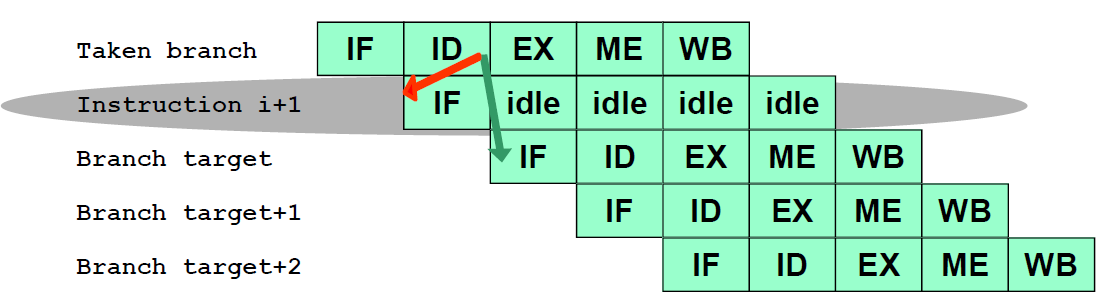
\includegraphics[scale=0.5]{img/branchpenality.png}
\caption{Esempio di penalità dovuto ad una predizione sbagliata}\label{fig:bantpenality}
\end{figure}
\paragraph{Branch Always Taken}
In alternativa al tipo di predizione precedente si può considerare che ogni salto sia sempre eseguito. Ogni qualvolta che un salto è decodificato e il suo indirizzo di destinazione è calcolato allora si assume che il salto sia eseguito e si introducono nella pipeline le istruzioni puntate dall'indirizzo di destinazione. Questo tipo di previsione ha senso in quelle pipeline dove l'indirizzo target è calcolato prima della comparazione dei registri.\\
Nelle pipeline di tipo MIPS noi non conosciamo l'indirizzo di destinazione prima della valutazione delle condizioni di salto così non vi è alcun vantaggio dall'utilizzo di questa tecnica.
\paragraph{Backward Taken Forward Not Taken (BTFNT)}
La predizione di questa tecnica si basa sulla direzione del salto, ovvero se i salti sono all'indietro sono previsti come eseguiti (come ad esempio nei cicli) salti in avanti sono considerati come non eseguiti.
\paragraph{Profile-driven Prediction}
Questo tipo di predizione si basa su dati raccolti da precedenti esecuzioni del programma utilizzando alcune funzioni del compilatore.
\paragraph{Delayed Branch Technique}
In questo tipo di tecnica il compilatore schedula una particolare istruzione indipendente dal salto in un campo chiamato \textbf{branch delay slot}. L'istruzione in questo slot viene eseguita ogni qualvolta che  il salto viene eseguito oppure no. Se assumiamo il ritardo dovuto ad un salto pari ad un ciclo di clock allora gli slot necessari per le istruzioni sono uno.
Un esempio di questa tecnica è mostrato in \figurename\,\ref{fig:branchdelay} dove nel \emph{branch delay slot} viene inserita un'istruzione di \texttt{add} indipendente dal ciclo.
\begin{figure}[htb]
\centering
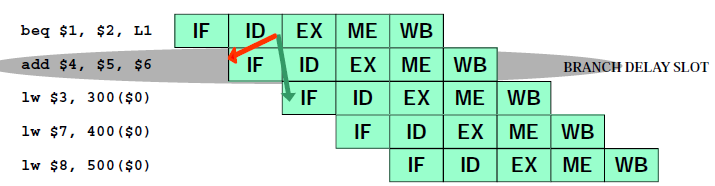
\includegraphics[scale=0.5]{img/branchdelay.png}
\caption{Esempio di utilizzo del branch delay slot}\label{fig:branchdelay}
\end{figure}
Sia nel caso che il salto sia eseguito sia nel caso non sia eseguito l'istruzione dopo quella di salto è sempre quella del \emph{delay slot} tuttavia nel caso il salto sia eseguito dopo l'istruzione del \emph{delay slot} l'esecuzione prosegue con le istruzioni del salto viceversa nel caso non sia eseguito allora l'esecuzione prosegue con le istruzioni successive.\\
Il compilatore deve essere in grado di selezionare l'istruzione da inserire nel delay slot in modo che essa sia valida ed utile. Ci sono quattro modi per selezionare tale istruzione:
\begin{itemize}
\item From Before
\item From Target
\item From Fall-Through
\item From After
\end{itemize}
La tecnica \emph{From Before} prevede di selezionare un istruzione indipendente selezionata tra quelle che precedono il salto in tale modo l'istruzione viene sempre eseguita. Il metodo \emph{From Target} prevede la copia dell'istruzione puntata dal salto; questa tecnica è preferibile quando il salto ha un alta probabilità di essere eseguito. Un esempio di utilizzo di questa tecnica è mostrato in \figurename\,\ref{fig:fromtarget}.
\begin{figure}[htb]
\centering
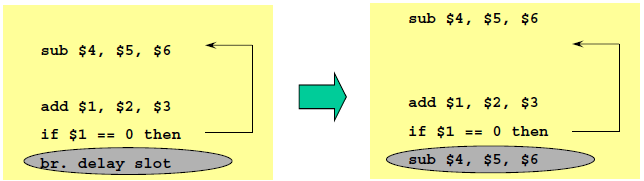
\includegraphics[scale=0.5]{img/fromtarget.png}
\caption{Esempio di selezione dell'istruzione \emph{From Target}}\label{fig:fromtarget}
\end{figure}
La tecnica \emph{From Fall-Through} e contrapposta alla tecnica \emph{From Targhet} infatti questa prevede che l'istruzione selezionata per il delay slot sia la prima istruzione che verrebbe prelevata nel caso di salto non eseguito come si vede dalla \figurename\,\ref{fig:fromfall}
\begin{figure}[htb]
\centering
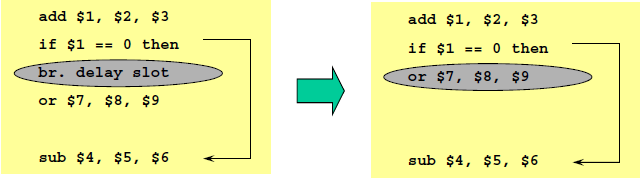
\includegraphics[scale=0.5]{img/fromfall.png}
\caption{Esempio di uso della tecnica \emph{From Fall-Through}}\label{fig:fromfall}
\end{figure}
Questo tipo di tecnica è preferibile quando il salto ha un alta probabilità di essere non eseguito.
Perchè le ultime due tecniche risultino corrette è necessario che le istruzioni eseguite quando il salto non prende la direzione prevista risultino ininfluenti rispetto alla normale esecuzione del programma. Questo è possibile ad esempio se l'istruzione nel delay slot agisce su dei registri che sono inutilizzati nel caso di risultato inaspettato del salto.\\
In generale il compilatore è in grado di assegnare il 50\% dei \emph{delay slot} con istruzioni valide e utili, all'altro 50\% viene riempito con istruzioni di tipo \texttt{nop}. Nel caso di pipeline più profonda il tempo necessario per valutare il salto è maggiore di un ciclo di clock e di conseguenza aumenta il numero di delay slot da riempire; diventa sempre più difficile perciò riempire tali slot con istruzioni valide e utili. Le principali limitazioni che nascono sono dovute alle restrizioni sulle istruzioni che possono essere schedulate e sull'abilità del compilatore di predire staticamente il risultato del salto.\\
Per migliorare l'abilità del compilatore di riempire i \emph{delay slot} molti processori hanno introdotto il \textbf{canceling or nullifing branch} ovvero salti nei quali è anche compresa la predizione della direzione del salto. Quando la predizione è verificata allora il contenuto del \emph{delay slot} è eseguito in caso contrario viene eseguita una \texttt{nop}
\subsubsection{Tecniche di predizione dinaminche}
L'idea di base in questo tipo di tecnica è quella di utilizzare il risultato di esecuzioni di salti passate per predire i salti futuri. Possiamo utilizzare dell'hardware per predire dinamicamente il risultato del salto; la predizione dipende dal comportamento dei salti durante l'esecuzione.\\
Il meccanismo di predizione dinamica si basa su due meccanismi che interagiscono tra loro:
\begin{itemize}
\item \textbf{Branch Outcame Predictor:} che tenta di predire la direzione del branch.
\item \textbf{Branch Target Predictor:} che calcola l'indirizzo di destinazione del salto nel caso in cui la condizione del salto abbia un risultato positivo.
\end{itemize}
Questi due moduli sono usate dall'unità di Instruction Fetch per predire la prossima istruzione da prelevare dall'I-Cache. Nel caso in cui il salto non venga eseguito il PC viene semplicemente incrementato, nel caso in cui, invece il branch venga preso il branch target predictor fornisce l'indirizzo di destinazione. Esiste inoltre una tabella chiamata \textbf{Branch History Table}  la quale contiene un bit per ogni predizione passata che indica se il salto è stato preso oppure no. L'indice della tabella è basato su di una piccola porzione dell'indirizzo dell'istruzione di salto. Se la previsione è corretta e si prosegue nella direzione della previsione. Se la previsione risulta sbagliata il bit di previsione viene invertito e riportato nella tabella. Ogni accesso in tabella è un \emph{hit} anche se tuttavia il bit di predizione può essere stato modificato da un altro salto con la stessa porzione di indirizzo.
\begin{figure}[htb]
\centering
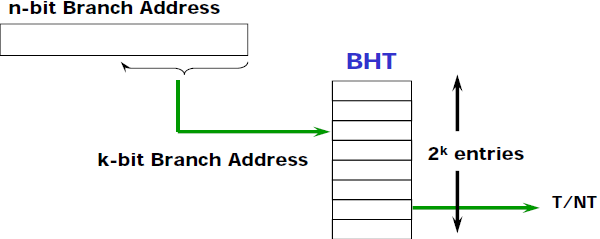
\includegraphics[scale=0.5]{img/historytable.png}
\caption{Esempio di \emph{Branch History Table}}\label{fig:historytable}
\end{figure}
Una predizione errata avviene quando una predizione risulta sbagliata oppure quando un indice è puntato da due differenti salti e la previsione si riferisce all'altro salto, per risolvere questo problema è sufficiente incrementare il numero di righe della BHTo utilizzare una funzione di hash.\\
Nel caso di una BHT ad un solo bit e considerando per esempio un salto di un loop che solitamente è eseguito la BHT sbaglierà predizione due volte, nel caso non sia eseguito e nel caso in cui venga eseguito il salto subito dopo non essere stato eseguito. Per meglio specificare i due casi abbiamo:
\begin{itemize}
\item All'ultima iterazione quando il salto non viene eseguito anche se la predizione indicava il contrario
\item Quando rientriamo nel loop alla fine della prima interazione la nostra predizione indica che dovremmo uscire (ultima interazione del loop precedente) mentre in realtà effettueremo il salto. 
\end{itemize}
Per ovviare a questo problema sfruttiamo una BHT a due bit nella quale sono necessarie due predizioni sbagliate consecutive per cambiare la nostra predizione. Per ogni indice della tabella i due bit sono utilizzati per indicare un dei quattro stati della macchina a stati finita in \figurename\,\ref{fig:bhtfsm}
\begin{figure}[htb]
\centering
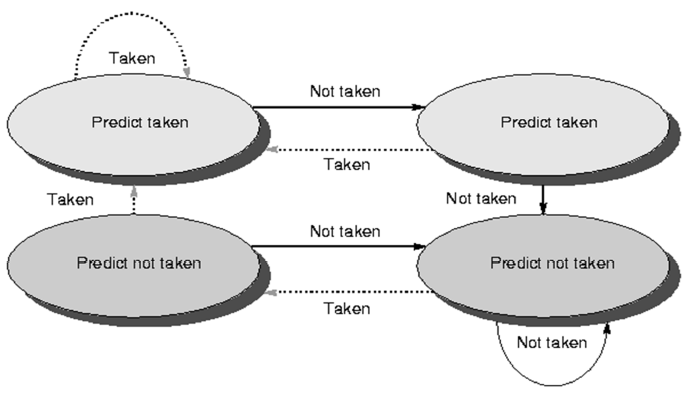
\includegraphics[scale=0.4]{img/bhtfsm.png}
\caption{Macchina a stati finita per una BHT a 2 bit}\label{fig:bhtfsm}
\end{figure}
Tale tecnica si può generalizzare fino ad utilizzare una tabella con \emph{n} bit per ogni record. Il valore che può assumere questo record va da 0 a $2^n-1$; quando il valore del record diventa uguale ad almeno la metà del suo valore massimo ($2^n-1$) la predizione del salto indica che esso deve essere eseguito, altrimenti la predizione sarà che non deve essere eseguito. Nello schema precedente il contatore veniva incrementato quando il salto veniva intrapreso e decrementato quando non veniva intrapreso.
\\ Tuttavia anche se una generalizzazione è possibile gli studi hanno dimostrato che una una tabella a 2 bit fornisce dati più che soddisfacenti. Ad esempio per una architettura IBM \emph{SPEC89} con una BHT con 4K record di 2 bit l'accuratezza nella predizione varia dal $99\%$ all'$82\%$.\\
La BHT a 2 bit utilizza solo i risultati delle esecuzioni precedenti di un singolo salto per predire il risultato di quel salto. L'idea di base però è che il comportamento dei salti recenti è che essi sono correlati con il comportamento di altri salti e perciò la predizione può essere influenzata da tali comportamenti. Un esempio è mostrato in \figurename\,\ref{fig:correletedbranch}
\begin{figure}[htb]
\centering
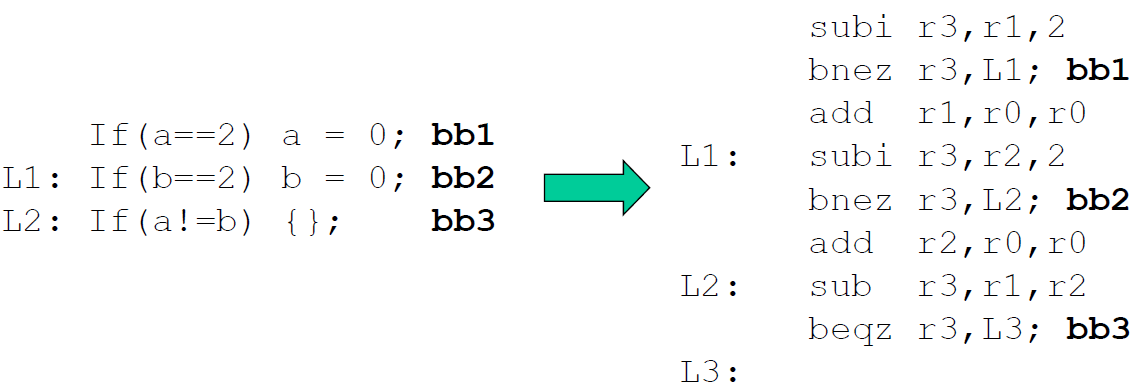
\includegraphics[scale=0.5]{img/correleted.png}
\caption{Esempio di salti correlati}\label{fig:correletedbranch}
\end{figure}
Un predittore che utilizza il comportamento di altri salti per effettuare una predizione è chiamato \textbf{Correlating  Predictors} o anche \textbf{2-Level Predictors}.
Un esempio di un \emph{(1,1) Correlating Predictors} è un predittore ad un bit con un bit di correlazione, ovvero il comportamento dell'ultimo salto è utilizzato per scegliere una coppia di predittori ad un bit come mostrato in \figurename\,\ref{fig:11correlato}.
\begin{figure}
\centering
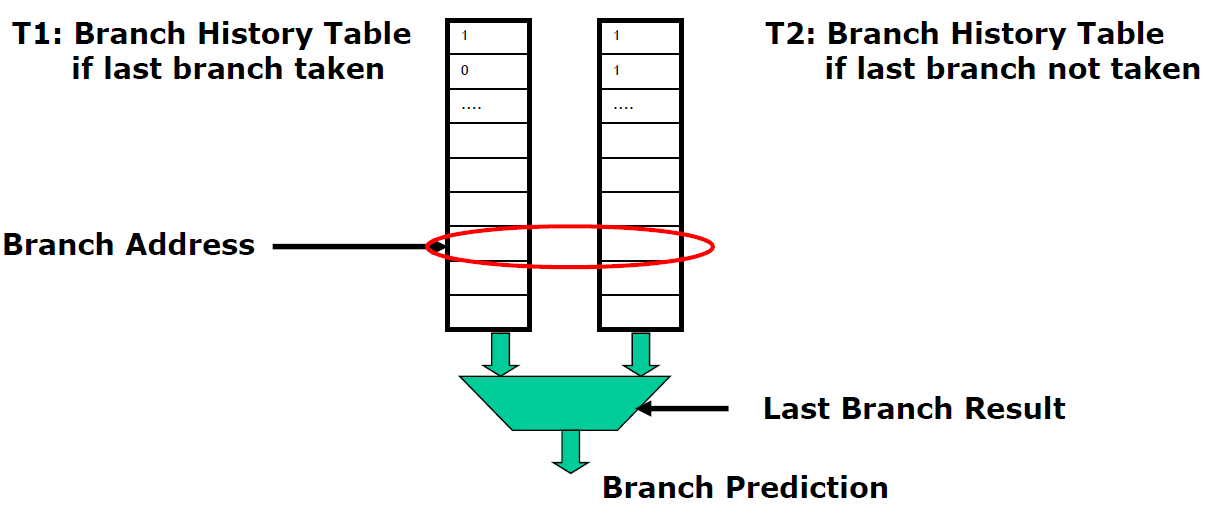
\includegraphics[scale=0.5]{img/11correlato.png}
\caption{Esempio di predittore correlato di tipo (1,1)}\label{fig:11correlato}
\end{figure}
Si registrano le esecuzioni degli ultimi k salti; la predizione si basa sull'esecuzione del salto precedente selezionando la BHT ad un bit appropriata:
\begin{itemize}
\item Una predizione è usata nel caso in cui l'ultimo salto è stato eseguito.
\item L'altra predizione è utilizzata se l'ultimo salto non è stato intrapreso.
\end{itemize}
In generale l'esecuzione dell'ultimo salto non riguarda la stessa istruzione sulla quale si cerca di fare una predizione come normalmente accade nei loop semplici.\\
In generale possiamo costruire un predittore correlato con (m,n) dove \emph{m} indica gli ultimi \emph{m} salti da analizzare selezionando $2^m$ BHT ognuna delle quali è un predittore a \emph{n} bit.
Il branch prediction buffer può essere indicizzato concatenando la parte finale del branch address con gli \emph{m} bit della \emph{global history}.
Un esempio di un predittore correlato è un predittore (2,2) dove si hanno quattro BHT a 2 bit tra i quali sceglieree si usano 2 bit dalla global history per selezionare quale utilizzare come mostrato in \figurename\,\ref{fig:22correlato}
\begin{figure}[bht]
\centering
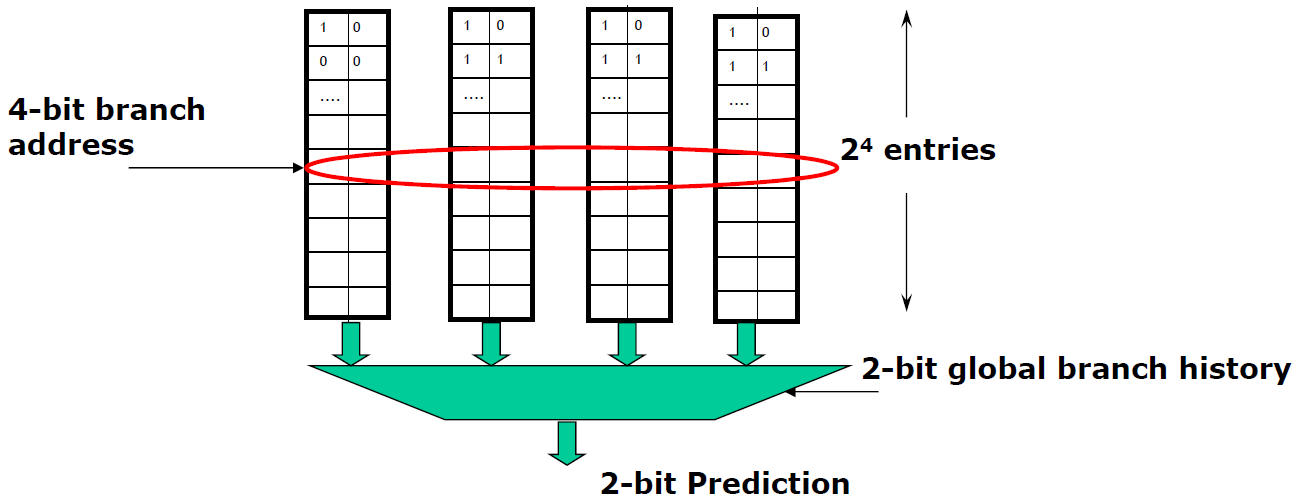
\includegraphics[scale=0.5]{img/22correlato.png}
\caption{Esempio di predittore correlato (2,2)}\label{fig:22correlato}
\end{figure}
Un predittore a due bit non correlato non è altro che un predittore correlato con i valori (0,2); a questo punto possiamo confrontare le performance nel caso di un predittore semplice a 2 bit con una tabella di 4K entità e un predittore correlato (2,2) con tabelle di 1K entità. Come vediamo dal grafico in \figurename\,\ref{fig:performance}
Il predittore correlato è, in molti casi più efficace di un predittore semplice mentre nei casi peggiori ne eguaglia le performance.
\begin{figure}[htb]
\centering
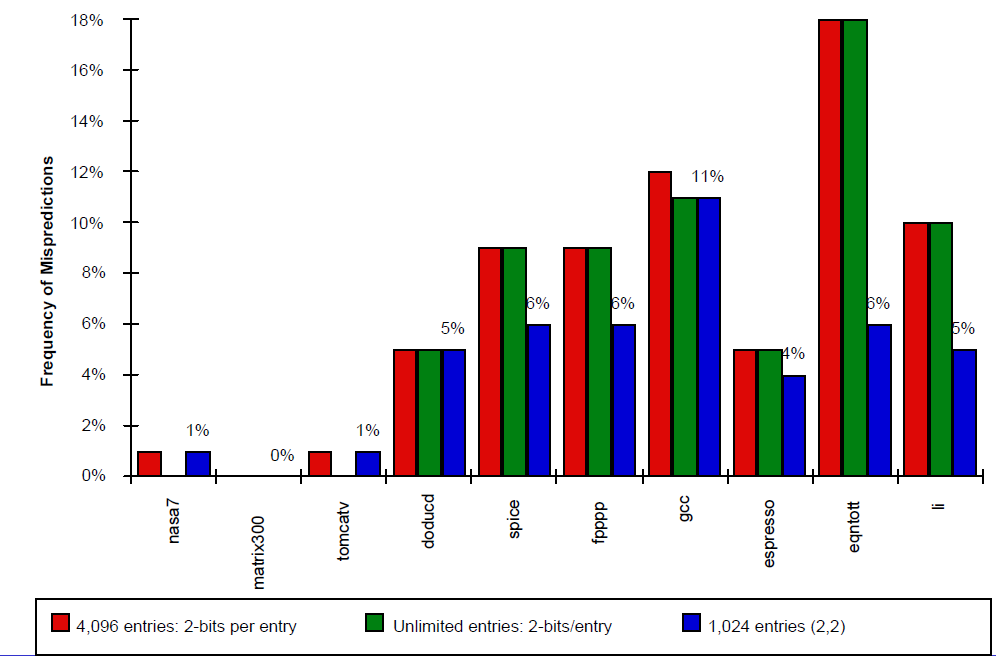
\includegraphics[scale=0.5]{img/performance.png}
\caption{Comparazione delle performance per predittore non correlato e predittore corellato}\label{fig:performance}
\end{figure}
Un altra tecnica di predizione dinamica è quella del \textbf{Predittore di salto adattativo a due livelli} (\emph{Two-Level Adaptative Branch Predictors}) nel quale un primo livello di storia viene memorizzato in uno shift register a \emph{k} bit chiamato \textbf{Branch History Register (BHR)} il quale memorizza i risultati degli ultimi k salti. Il secondo livello di storicizzazione è memorizzato in una tabella con record di due bit chiamata \textbf{Pattern History Table (PHT)} per indicare la predizione.
La BHR è utilizzata per indicizzare la PHT e selezionare i due bit da utilizzre; per selezionera quale dei due bit utilizzare si utilizza lo stesso principio utilizzato per i predittori a due bit semplici.
\begin{figure}[htb]
\centering
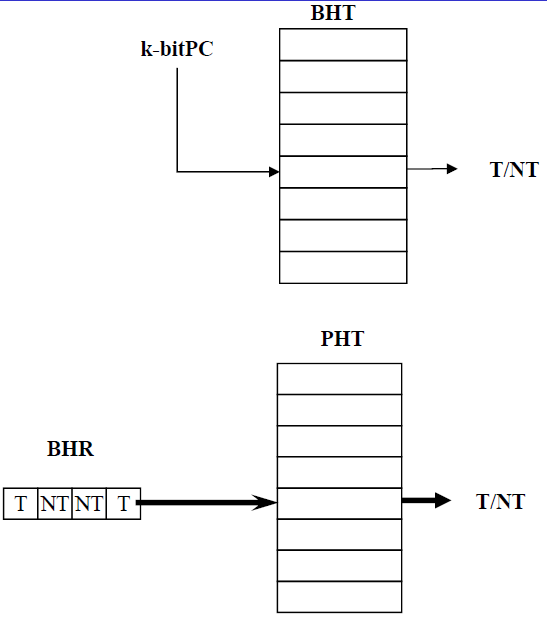
\includegraphics[scale=0.5]{img/gapred.png}
\caption{Esempio di predittore adattativo}\label{fig:gapred}
\end{figure}
Un evoluzione di questo predittore è il \textbf{predittore GShare} dove le informazioni dell'indirizzo locali vengono correlate con quelle globali tramite un'operazione di XOR.
\begin{figure}[htb]
\centering
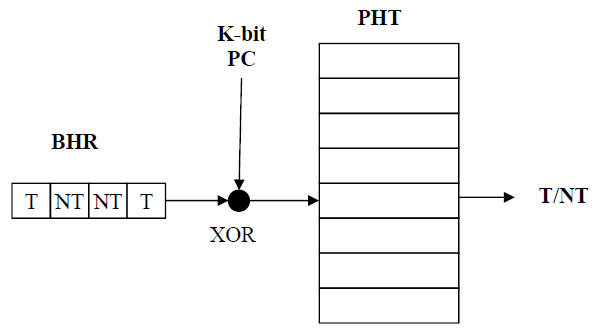
\includegraphics[scale=0.5]{img/gshare.png}
\caption{Esempio di predittore GShare}\label{fig:gshare}
\end{figure}
Un ultimo elemento importante nella predizione dinamica è il \textbf{Branch Target Buffer} la quale è una cache nella quale vengono memorizzate l'indirizzo di destinazione del salto per le istruzioni dopo il salto. Accediamo al BTB nello stage IF utilizzando l'indirizzo dell'istruzione da prelevare per indicizzare la cache. Un possibile esempio di record è mostrato in \figurename\,\ref{fig:btbrecord}.
\begin{figure}[htb]
\centering
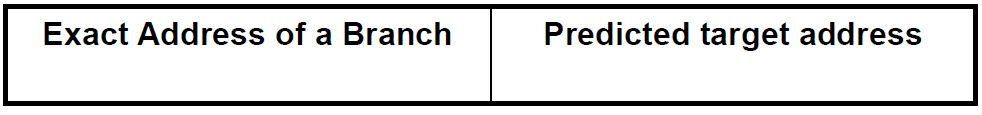
\includegraphics[scale=0.5]{img/btbrecord.png}
\caption{Esempio di record di un Branch Target Buffer}\label{fig:btbrecord}
\end{figure}
L'indirizzo di destinazione  del salto è espresso sempre in modo relativo al PC.
La struttura del BTB è mostrata in \figurename\,\ref{fig:btbstrut}; in tale buffer dobbiamo memorizzare solo gli indirizzi per quei salti che vengono eseguiti.
\begin{figure}[htb]
\centering
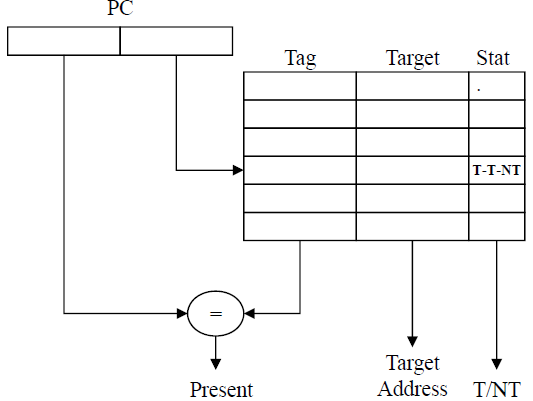
\includegraphics[scale=0.5]{img/btbstrut.png}
\caption{Struttura di un Branch Target Buffer}\label{fig:btbstrut}
\end{figure}
\subsection{Speculazione}
Senza tecniche di predizione di salto il parallelismo risulta molto limitato e si riduce all'analisi dei \textbf{basic block} ovvero a pezzi di codice nei quali non entrano o escono dei salti. Tuttavia possiamo azzardare alcune supposizioni di parallelismo tra diversi blocchi base effettuando delle speculazioni. Tramite le speculazioni possiamo recuperare ed eseguire le istruzioni come se le nostre predizioni siano corrette gestendo in seguito il caso in cui non siano corrette. Tale speculazione può essere supportata sia dal compilatore che dall'hardware.
%\section{Instruction Level Parallelism}\label{capitolo3}
Come abbiamo visto nei capitoli precedenti in una macchina fornita di pipeline possiamo dimostrare come il numero di clock necessari per eseguire un'istruzione sia:
$$\begin{array}{rcl}
CPI_{pipeline} & = & CPI_{ideale}+ Stalli \ Strutturali + Stalli \ Data \ Hazard + \\
&& Stalli \ di \ Controllo + Stalli \ di \ Memoria
\end{array}$$
La riduzione di uno qualsiasi dei termini sulla destra da in modo che $CPI_{pipeline}$ si avvicini sempre più al $CPI_{ideale}$. Il caso migliore si ha quando il throughput è massimo ed è uguale a 1
$$IPC_{ideale} = 1; \\ CPI_{ideale} = 1$$
Tuttavia si hanno dei limiti alle performance dovuti ai diversi tipi di \emph{rischi (Hazards)}, questi possono essere di diversa natura:
\begin{itemize}
\item \textbf{Strutturali:} si possono risolvere tramite l'introduzione di nuovo hardware.
\item \textbf{Dati:} necessitano di \emph{forwarding} e di una schedulazione del codice a livello di compilazione.
\item \textbf{Controllo:} Early evaluation, Branch Delay Slot, Predizione dei salti statica e dinamica.
\end{itemize}
Inoltre per le pipeline più profonde (superpipelining) questi problemi sono accentuati.\\
In questo capitolo ci concentreremo su come incrementare il \emph{CPI} oltre il valore ideale; per fare ciò però dobbiamo prima capire quali sono gli \emph{hazard} sui dati che possiamo incontrare.
\subsection{Tipi di Hazards sui dati}
Gli hazard innanzitutto sono quei conflitti che avvengono a tempo di esecuzioni e sono generati da dipendenze a livello di istruzione. Consideriamo l'esecuzione di un istruzione generale di questo tipo:
$$r_k \leftarrow (r_i) \ op \ (r_j)$$
Possiamo avere tre tipi di dipendenza a livello di istruzione come mostrato in \figurename\,\ref{fig:datadep}
\begin{figure}[htb]
\centering
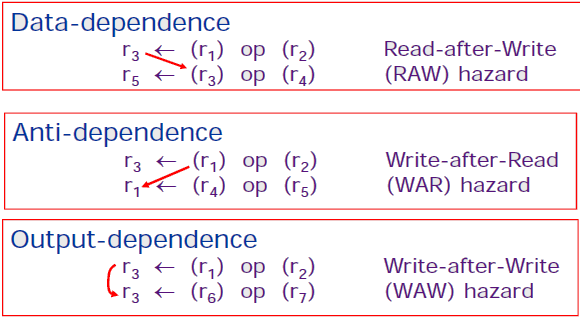
\includegraphics[scale=0.4]{img/datadep.png}
\caption{Esempi di dipendenza dei dati}\label{fig:datadep}
\end{figure}
\subsection{Parallelismo a livello di istruzione}
Per raggiungere livelli di performance maggiori è necessario estrarre dai programmi maggiore parallelismo, questo si traduce in pipeline con più uscite (\emph{multiple-issue}). Per fare ciò è necessario individuare e risolvere le dipendenze, inoltre è utile riordinare (\emph{schedule}) le istruzioni in modo da ottenere un maggiore parallelismo a tempo di esecuzione compatibilmente con le risorse a disposizione.\\
Per dare una definizione formale del parallelismo a livello di istruzione (\emph{ILP}) possiamo dire che 
\begin{center}
\textit{ILP = Sfruttare la potenziale esecuzione sovrapposta di istruzione non correlate}
\end{center}
Tale sovrapposizione è possibile tutte le volte che:
\begin{itemize}
\item Non abbiamo degli \emph{Hazard} di tipo strutturale
\item Non abbiamo \emph{Hazard} di tipo RAW, WAR oppure WAW
\item Non abbiamo \emph{Hazard} di controllo
\end{itemize}
Un esempio di sistema \emph{dual-issue} è mostrato in \figurename\,\ref{fig:dualpipe} e \figurename\,\ref{fig:dualmips}
\begin{figure}
\centering
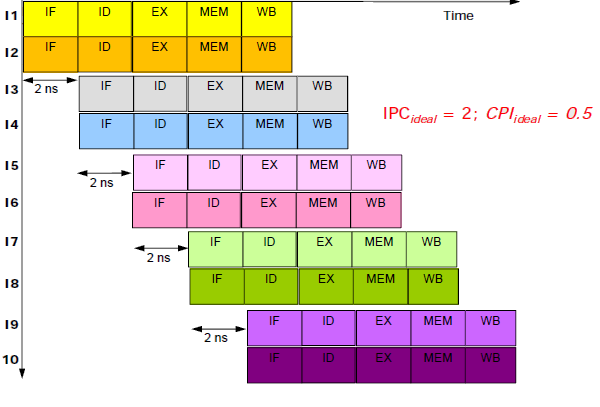
\includegraphics[scale=0.5]{img/dualpipe.png}
\caption{Esecuzione di istruzione in una pipeline dual-issue}\label{fig:dualpipe}
\end{figure}
\begin{figure}
\centering
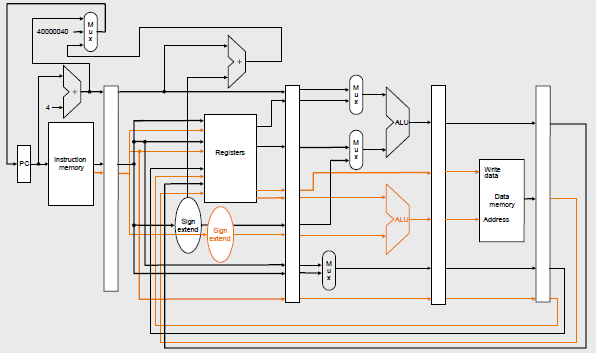
\includegraphics[scale=0.5]{img/dualmips.png}
\caption{Schema hardware per una pipeline dual-issue con una unità ALU/BR e una unità load/store}\label{fig:dualmips}
\end{figure}
In pipeline di tipo multiple-issue il $CPI_{ideale}$ risulta essere $<1$ ad esempio considerando il caso ottimale di un processore \emph{2-issue} abbiamo che ad ogni ciclo di clock vengono completate 2 istruzioni questo significa che:
$$IPC_{ideale} = 2; \\ CPI_{ideale} = 0.5$$
Uno degli aspetti più critici nel caso di ILP è la determinazione delle dipendenze tra le istruzioni; infatti, se due istruzioni sono dipendenti tra loro esse non possono essere eseguite in parallelo ma dovranno essere eseguite in sequenza o al più in parziale sovrapposizione. Possiamo distinguere tre tipi di dipendenza:
\begin{itemize}
\item Dipendenza dei dati (Vera dipendenza)
\item Dipendenza dei nomi
\item Dipendenza di controllo
\end{itemize}
\paragraph{Dipendenza dei nomi}
Tale dipendenza avviene quando due istruzioni usano lo stesso registro o la stessa area di memoria (chiamata \emph{nome}) ma non esiste alcun flusso di dati tra queste due istruzioni. Possiamo individuare due tipi di dipendenza dai nomi tra due istruzioni \textbf{i} e \textbf{j} nelle quali \textbf{i} precede \textbf{j}
\begin{itemize}
\item \textbf{Antidipendenza:} quando l'istruzione \emph{j} scrive un registro che l'istruzione \textbf{i} legge; l'ordine originale delle istruzioni deve essere preservato per essere sicuri che \textbf{i} legga il valore corretto (WAR).
\item \textbf{Output dipendenza:} quando \textbf{i} e \textbf{j} scrivono lo stesso registro o la stessa area di memoria; l'ordine delle istruzioni deve essere rispettato per essere sicuri che il valore finale sia quello scritto da \textbf{j}
\end{itemize}
In realtà la dipendenza dai nomi non è una vera e propria dipendenza in quanto non vi è alcuno scambio di valori tra le istruzioni; se il \emph{nome} usato nell'istruzione può essere cambiato non ci sono conflitti. Tuttavia per quanto riguarda le aree di memoria è molto più difficile localizzare questo tipo di conflitto infatti due indirizzi possono essere diversi ma puntare alla stessa area (\emph{memory disambiguation}) mentre una rinominazione dei registri risulta molto più semplice.
La rinominazione può essere effettuata sia staticamente dal compilatore sia in modo dinamico dall'hardware.
\paragraph{Dipendenze dei dati}
Le dipendenze dei dati possono potenzialmente generare dei \emph{Data Hazard} ma l'impatto che questi hazard hanno in termini di stalli e tecniche di eliminazione degli stalli sono caratteristiche specifiche della pipeline e non dipendono dalla dipendenza.
Le \emph{RAW} sono le uniche vere dipendenze sui dati che abbiamo.
Le dipendenze sono una caratteristica del programma mentre gli \emph{hazard} sono specifiche della pipeline.
\paragraph{Dipendenze di controllo}
Le dipendenze di controllo sono determinate dall'ordinamento delle istruzioni e sono preservate da due proprietà:
\begin{itemize}
\item Le istruzioni devono essere eseguite nell'ordine del programma per assicurare che un'istruzione che si trova prima di un salto venga eseguita prima del salto.
\item Individuazione degli \emph{hazard di controllo} per assicurare che un'istruzione che dipende da un salto non sia eseguita prima di conoscere la direzione del salto.
\end{itemize}
Sebbene preservare il controllo delle dipendenze sia un modo semplice per preservare l'ordine del programma esso non è così essenziale da dover essere preservato.
\subsubsection{ILP in pratica}
Dalla trattazione appena fatta possiamo ricavare due proprietà importanti per verificare la correttezza di un programma (e che in realtà preservano sia le dipendenze dei dati che quelle di controllo):
\begin{itemize}
\item \textbf{Data flow:} il flusso dei valori dei dati attraverso le istruzioni deve produrre il risultato corretto.
\item \textbf{Exception behavior:} preservare il comportamento delle eccezioni che significa che qualsiasi cambiamento nell'ordine di esecuzione delle istruzioni non deve cambiare come le eccezioni sono sollevate dal programma.
\end{itemize}
Esistono due tecniche fondamentali per supportare e implementare l'\emph{ILP}, lo \textbf{scheduling dinamico} che dipende dall'hardware per localizzare il parallelismo e lo \textbf{scheduling statico} che fa affidamento sul software per individuare possibili parallelismi. La prima soluzione è quella più utilizzata in ambito desktop e server.\\
Consideriamo ora un processore di tipo \emph{single-issue} lo stage IF precede quello EXE e le istruzioni possono essere prelevate sia dall'\emph{Instruction Register} sia da una coda di istruzioni pendenti. La fase di esecuzione può richiedere più cicli di clock in base al tipo di operazione.\\
\paragraph{Scheduling dinamico}
Il problema principale è quello che non si può nascondere una dipendenza dai dati senza causare uno stallo nell'esecuzione della pipeline. Una soluzione è quella di permettere alle istruzioni situate dopo lo stallo di procedere; l'hardware deve riordinare dinamicamente l'esecuzione delle istruzioni per dar in modo di ridurre gli stalli. Per fare ciò è necessario permettere un esecuzione fuori ordine e una fase di commit finale.\\
L'hardware riordina l'esecuzione delle istruzioni per ridurre il numero degli stalli della pipeline mentre mantiene il \emph{data flow} e \emph{exception behavior}. I vantaggi principali di questa tecnica sono il fatto di permettere una gestione di alcuni casi in cui esistono delle dipendenze non note al tempo della compilazione, inoltre permette di semplificare la complessità del compilatore ed infine permette di compilare il codice affinché esso venga eseguito efficientemente anche su pipeline diverse. Questi vantaggi tuttavia hanno un costo che comporta un significativo incremento della complessità dell'hardware, un incremento dei consumi e può generare delle eccezioni imprecisate.
Tale soluzione è utilizzata soprattutto nei \emph{Processori Super-scalari}
\paragraph{Scheduling statico}
In questo caso il compilatore utilizza dei sofisticati algoritmi per individuare e organizzare il codice in modo da sfruttare l'\emph{ILP}, per fare ciò analizza i \textbf{basic block} e ricerca il parallelismo in questi seppur esso sia minimo (15\% - 25\%), ed inoltre sfrutta il parallelismo tra diversi \emph{basic block}. Un limite a questa tecnica è però la dipendenza dai dati presente nei vari blocchi base. Tipicamente questa tecnica è sfruttata dai processori \textbf{VLIW} (\emph{Very Long Instruction Word}) i quali si aspettano del codice privo di dipendenze dal compilatore.\\
Il limite principale di questa tecnica è dato dall'impredicibilità dei salti, dalla latenza della memoria, dalla dimensione del codice e dalla complessità del compilatore.
\subsubsection{Esecuzione super-scalare e VLIW}
Passando al caso \emph{multi-issue} la questione si complica anche se le prestazioni migliorano come vediamo in \figurename\,\ref{fig:superscalar}, infatti si vogliono eseguire più istruzioni per ogni ciclo di clock; per fare ciò è necessario prelevare più istruzioni per ciclo dall'IR e questo dipende dalla banda a disposizione. La cosa più difficile però risulta essere l'analisi delle dipendenze dei dati e di controllo per le istruzioni da eseguire.
\begin{figure}[htb]
\centering
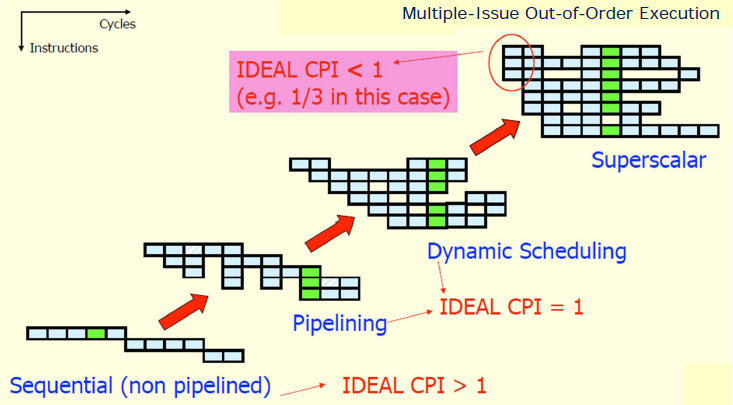
\includegraphics[scale=0.5]{img/superscalar.png}
\caption{Confronto di prestazioni tra architetture}\label{fig:superscalar}
\end{figure}
In \figurename\,\ref{fig:superstrut} vediamo come è strutturato un processore super-scalare nel quale possiamo notare le diverse unità per l'esecuzione di istruzioni parallele come le due ALU o l'unità per le istruzioni di load/store, e l'unità per il riordino delle istruzioni.\\
\begin{figure}[htb]
\centering
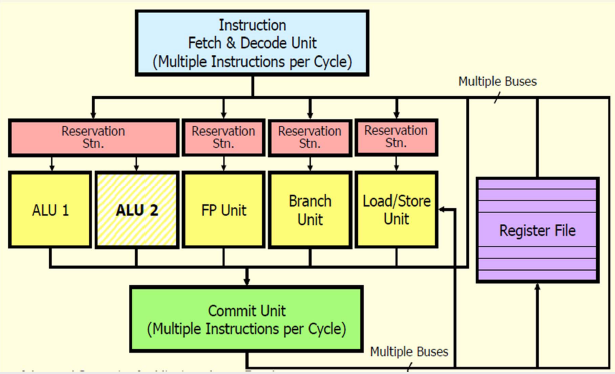
\includegraphics[scale=0.5]{img/superstrut.png}
\caption{Struttura di un prcessore superscalare}\label{fig:superstrut}
\end{figure}
Per decidere quali istruzioni mandare in esecuzione si utilizza lo \emph{Scheduler dinamico} il quale per ogni ciclo di clock analizza quali sono le dipendenze e per fare ciò la sua complessità è molto alta, nell'ordine del quadrato delle possibili istruzioni come mostrato in \figurename\,\ref{fig:dinamicscheduler}.
\begin{figure}[htb]
\centering
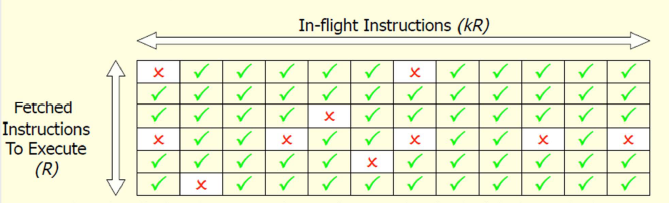
\includegraphics[scale=0.5]{img/dinamicscheduler.png}
\caption{Tabella delle dipendenze in uno scheduler dinamico}\label{fig:dinamicscheduler}
\end{figure}
Esiste un limite al numero di istruzioni che possono essere analizzate durante un singolo ciclo di clock, infatti i limiti principali dei processori super-scalari riguardano tutti lo scheduler dinamico in quanto esso è molto costoso in termini di area in quanto la sua logica è molto complessa, il tempo di clock dipende dal tempo di analisi delle istruzioni ed infine la verifica del design dello scheduler è molto complessa.
Queste limitazioni portano a delle limitazioni in termini di istruzioni che possono essere eseguite simultaneamente. Attualmente in realtà esistono dei processori a 6-issue anche se molto rari, più normalmente sono di tipo 4-issue o minori in quanto è troppo difficile trovare 8 o addirittura 16 istruzioni indipendenti in un singolo ciclo.\\
La famiglia di processori multi-issue che sfruttano lo scheduler statico sono, invece, i processori VLIW (\emph{Very Long Instruction Word}) nei quali è il compilatore che decide cosa far fare ad ogni istruzione per ogni ciclo di clock come si vede in \figurename\,\ref{fig:vliw}.
\begin{figure}[htb]
\centering
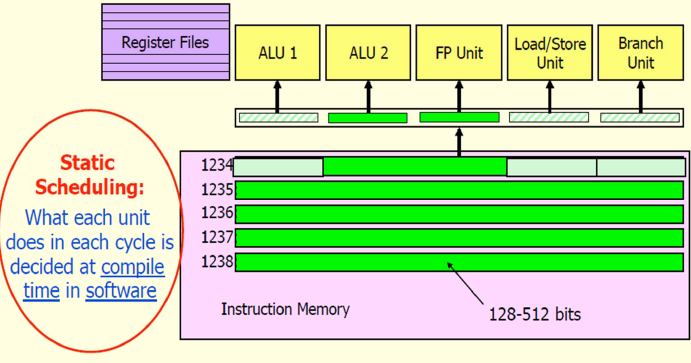
\includegraphics[scale=0.5]{img/vliw.png}
\caption{Scheduler statico nel caso di processori VLIW}\label{fig:vliw}
\end{figure}
I processori di tipo super-scalare sono utilizzati soprattutto in ambito desktop e server, mentre i processori VLIW sono utilizzati soprattutto in ambito embedded in quanto la decisione sull'esecuzione è presa a compile-time e non è necessario aggiungere dell'area per lo scheduler dinamico.
\subsection{Scoreboard}
Come abbiamo visto fino ad ora lo scheduling dinamico è il meccanismo più utilizzato nei sistemi general purpose per sfruttare il parallelismo tra le istruzioni. Tale meccanismo però ha diverse tecniche di implementazione, una di queste è lo \textbf{Scoreboard}. Lo \emph{Scoreboard} divide il normale stage ID in due stage per permettere l'esecuzione delle istruzioni nell'ordine più efficiente. Questi due stage sono:
\begin{itemize}
\item Lo stage \emph{issue} che si occupa di decodificare le istruzioni e di verificare eventuali hazard strutturali.
\item Lo stage \emph{read operands} (RR) che si occupa di risolvere i data hazard ritardando eventualmente la lettura dei registri.
\end{itemize}
Grazie a questo meccanismo le istruzioni vengono eseguite quando non hanno alcuna dipendenza o non esistono degli hazard strutturali non verifica però una eventuale priorità delle istruzioni.\\
Per spiegare la struttura dello \emph{Scoreboard} dobbiamo innanzitutto definire quando un'istruzione si dice in \textbf{esecuzione}. Possiamo distinguere quando un'istruzione inizia la sua esecuzione e quando essa la termina durante questi due istanti l'istruzione si dice in \emph{esecuzione}. In una pipeline possono esistere molte istruzioni in esecuzione nello stesso momento, questo richiede che esistano più unità funzionali. Quello che noi analizzeremo è la struttura di un \textbf{CDC 6600} nel quale le istruzioni vengono immesse in ordine ma vengono eseguite e completate in un ordine casuale. L'architettura di questo sistema è mostrata in \figurename\,\ref{fig:scorearch}
\begin{figure}[htb]
\centering
\includegraphics[scale=0.5]{img/scorearch.png}
\caption{Architettura di un sistema \emph{Scoreboard}}\label{fig:scorearch}
\end{figure}
Nella pipeline di uno scoreboard le fasi ID, EXE e WB sono sostituite da quattro stage. Lo stage ID è diviso in due parti, la prima chiamata \textbf{Issue} la quale decodifica l'istruzione e controlla eventuali hazard strutturali, la seconda chiamata \textbf{Read Operands} che attende fino alla risoluzione degli hazard sui dati. Lo scoreboard fa in modo che le istruzioni eseguite siano prive di dipendenze. Come abbiamo visto le istruzioni vengono prelevate in ordine dallo stage \emph{Issue} ma da quell'istante esse possono essere ordinate in qualsiasi modo, infatti durante lo stage \emph{read operands} esse possono essere bloccate o bypassate, inoltre, la latenza di esecuzione può variare tra le diverse unità funzionali.\\
Un completamento fuori ordine può portare però a hazard di tipo WAR o WAW che tuttavia possono essere facilmente risolti infatti per i WAR è sufficiente:
\begin{itemize}
\item Bloccare il \emph{write back} finché i registri non vengono letti
\item Effettuare la lettura dei registri soltanto durante la fase di \emph{Read Operands}
\end{itemize}
Mentre per risolvere i WAW è sufficiente individuare l'hazard e bloccare l'esecuzione delle istruzioni dipendenti successive fino a quando esse non vengono concluse.\\
L'individuazione e la risoluzione degli hazard è centralizzata nello \emph{scoreboard}; ogni istruzione attraversa lo scoreboard dove viene aggiornata una tabella delle dipendenze, a questo punto lo scoreboard determina quando l'istruzione può leggere i registri ed iniziare la sua esecuzione. Se un'istruzione non può cominciare immediatamente la sua esecuzione lo scoreboard monitora ogni cambiamento e decide quando l'istruzione può andare in esecuzione. Infine, lo scoreboard, controlla quando l'istruzione scrive il risultato dentro i registri di destinazione.\\
Un problema che si viene a creare quando si accetta il completamento delle istruzioni fuori ordine è quello della preservazione del comportamento delle eccezioni; una soluzione è quella di assicurarsi che nessuna istruzione possa generare una eccezione finché il processore non conosce esattamente l'istruzione che ha sollevato l'eccezione. Un'eccezione si dice \emph{imprecisa} se lo stato del processo nell'istante in cui viene sollevata una eccezione non è uguale a quello del caso in cui l'istruzione sia eseguita in ordine; un'eccezione imprecisa si può verificare quando la pipeline ha già completato delle istruzioni che sequenzialmente si trovano dopo l'istruzione che ha sollevato l'eccezione, oppure se non ha ancora completato istruzioni che sequenzialmente la precedono.
\paragraph{I quattro stadi dello Scoreboard}
Analizziamo ora in dettaglio i quattro stadi dello Scoreboard. Il primo stadio è quello di \emph{Issue} nel quale le istruzioni vengono decodificate e si verificano gli eventuali hazard strutturali e quelli di WAW. Le istruzioni lasciano questo stage in ordine, se l'unità funzionale necessaria per eseguire l'istruzione è libera e non esistono altre istruzioni che hanno lo stesso registro di destinazione (no WAW) lo stage issue inoltra l'istruzione all'unità funzionale e aggiorna la sua struttura interna. In caso contrario lo stage ferma l'istruzione fino a quando tutti gli hazard sono stati risolti. Ogni qualvolta lo stage di issue ferma un istruzione il buffer tra IF e Isuue si riempe. Nel caso il buffer sia singolo IF si blocca e attende l'Issue nel caso invece il buffer sia a coda l'IF si blocca solo nel caso in cui la coda sia piena.\\
Lo stage \emph{Read Operands} attende la risoluzione dei data hazard e legge i registri. Un registro risulta disponibile quando non ci sono istruzioni attive precedenti che scrivono su di esso oppure se un unità funzionale scrive il suo risultato in tale registro. Quando i registri sono disponibili lo scoreboard comunica all'unità funzionale di leggere i registri. Gli RAW hazard vengono risolti dinamicamente in questa fase.\\
Lo stage \emph{execution} è lo stage composto dalle unità funzionali; durante questo stage le unità funzionali svolgono le diverse operazioni, quando il risultato è pronto viene notificato allo scoreboard. Le unità funzionali sono caratterizzate da una latenza variabile, il tempo per iniziare l'esecuzione è variabile in quanto è il tempo necessario per leggere i diversi registri, i tempi per effettuare una load/store variano in base ai cache HIT/MISS.\\
L'ultimo stage è denominato \emph{Write Result}, in questa fase si controllano eventuali hazard di tipo WAR e si termina l'esecuzione scrivendo il risultato nel registro di destinazione.
\paragraph{Lo Scoreboard in pratica}
Lo scoreboard è formato da tre unità fondamentali:
\begin{itemize}
\item Instruction status
\item Functional Unit status: il quale indica lo stato delle unità fondamentali tramite diversi indici
\begin{description}
\item[Busy:] indica se la FU è occupata oppure no
\item[Op:] indica l'operazione da eseguire
\item[$F_i$:] registro di destinazione
\item[$F_j,F_k$:] registri sorgenti
\item[$Q_j,Q_k$:] indicano quale FU sta tenendo occupato il registro corrispondente
\item[$R_j,R_k$:] sono dei flag che indicano lo stato dei registri sorgenti.
\end{description}
\item Register Result status: indica quale FU dovrà scrivere sui registri di destinazione.
\end{itemize}
Per un esempio completo si rimanda alle slide dell'insegnante.
\subsection{Algoritmo di Tomasulo}
Un altro tipo di algoritmo da sfruttare per lo scheduling dinamico è l'algoritmo di \emph{Tomasulo} introdotto da IBM tre anni dopo il CDC 6600 lo scopo di tale algoritmo è sempre quello di ottenere prestazioni elevate senza l'utilizzo di speciali compilatori.\\
A differenza dello Scoreboard tuttavia il meccanismo di controllo e di buffer è distribuito sulle diverse unità funzionali. I buffer associati alle unità funzionali sono chiamate \emph{Reservation Station}. I registri nelle istruzioni sono sostituiti da valori o puntatori alle reservation station è possibile così il renaming dei registri. In questo modo si evitano anche eventuali hazard di tipi WAR e WAW; inoltre esistono più \emph{RS} che registri e questo permette delle ottimizzazioni che il compilatore non può fare. Infine il risultato delle FU non transita dai registri bensì viene diffuso a tutte le altre FU tramite un \emph{Common Data Bus}. Le operazioni di Load e Store sono trattate come normali FU . L'architettura necessaria per implementare l'algoritmo di Tomasulo è mostrata in \figurename\,\ref{fig:tomahw} mentre la struttura di una unità funzionale è mostrata in \figurename\,\ref{fig:fuhw}
\begin{figure}
\centering
\includegraphics[scale=0.5]{img/tomahw.png}
\caption{Architettura per l'algoritmo di Tomasulo}\label{fig:tomahw}
\end{figure}
\begin{figure}
\centering
\includegraphics[scale=0.5]{img/fuhw.png}
\caption{Architettura di un'unità funzionale}\label{fig:fuhw}
\end{figure}
I vari campi che compongono una reservation station sono:
\begin{description}
\item[Tag:] identifica quale RS è coinvolta.
\item[Busy:] identifica se la RS è occupata.
\item[OP:] Identifica il tipo di operazione eseguita dal componete.
\item[$V_j,V_k$:] Valori contenuti nei registri; per la \emph{load}  $V_j$ contiene il valore dell'offset.
\item[$Q_j,Q_k$:] Puntatori alle RS che producono i valori $V_j,V_k$ se il valore è uguale a 0 l'operando è già disponibile. 
\end{description}
Si noti che solo uno dei due campi \emph{V} e \emph{Q} è disponibile per ogni operando in un determinato istante.\\
Il register file e lo Store buffer hanno un campo \emph{Value (V)} e uno \emph{Puntatore (Q)} il quale punta al numero della \emph{reservation station} che produce il risultato da immagazzinare, se questo puntatore è uguale a zero allora non ci sono istruzioni attive e il valore contenuto nel RF/Buffer è quello corretto.
Nel caso di Load buffer abbiamo un campo \emph{Address (A)} e un campo \emph{Busy}; il campo \emph{A} mantiene le informazioni riguardanti gli indirizzi calcolati nelle operazioni di Load/Store, all'inizio contiene le informazioni sull'offset poi, una volta calcolato, contiene l'indirizzo effettivo.
\subsubsection{Gli stadi dell'algoritmo di Tomasulo}
\paragraph{Il primo stadio: ISSUE}
Durante questo stadio si preleva un'istruzione \emph{I} dalla testa della coda delle istruzioni (\textbf{in-order issue}). Si controlla se la RS associata a quell'istruzione è vuota altrimenti si attende (controllo sugli structural hazard). Nel caso gli operandi non siano ancora disponibili si tiene traccia della FU che produce tali operandi (puntatore Q). Durante questa fase si effettua anche il \emph{Rename} dei registri in modo tale da evitare eventuali \emph{WAR}, infatti, se un istruzione \emph{I} scrive un registro \emph{$R_x$} e un istruzione $K$ già prelevata legge tale registro $K$ conosce già il valore di $R_x$ e lo ha immagazzinato nella sua RS oppure conosce quale operazione produce tale valore. Inoltre si evitano anche eventuali WAW in quanto le istruzioni sono prelevate in ordine.
\paragraph{Secondo stadio: Esecuzione}
Quando entrambi gli operandi sono disponibili si esegue l'operazione; nel caso in cui non siano pronti invece si controlla il \emph{Common Data Bus} in attesa del risultato; ritardando l'esecuzione si evitano eventuali RAW. Si noti come più istruzioni possono diventare eseguibili allo stesso istante per la stessa FU a questo punto bisogna verificare la disponibilità dell'unità funzionale. Le RAW hazard sono molto meno incisive in quanto sono gestite a livello di RS e non è necessario attendere il \emph{write back} sul register file.\\
Per quanto riguarda le istruzioni di load e di store l'esecuzione avviene in due passi, nel primo passo si calcola l'effettivo indirizzo di destinazione e si memorizza nel buffer, nel secondo passo in caso di load si esegue l'operazione non appena l'unità è disponibile nel caso della store si attende invece che il dato da immagazzinare sia disponibile.\\
Per preservare il comportamento dell'esecuzione nessuna istruzione può cominciare l'esecuzione fino a quando i branch precedenti non sono stati eseguiti. Se si usano tecniche di predizione la CPU deve conoscere se la predizione è corretta prima di procedere.
\paragraph{Terzo stadio: Write result}
Quando un risultato è disponibile esso viene scritto sul \emph{Common Data Bus} e da qui copiato sia sul RF sia su tutte le RS che attendono questo risultato. Il \emph{Common Data Bus} è un bus di tipo data+source composto da 64 bit di dati e 4 bit per la sorgente in questo modo le FU possono effettuare un lookup associativo.
\subsubsection{Alcuni dettagli}
Le operazioni di load e di store attraversano un'unità funzionale per il calcolo dell'indirizzo effettivo prima di procedere con le vere e proprie operazioni di load e di store. La load necessita di una seconda fase per accedere alla memoria mentre invia il risultato al RF e alle RS durante lo stage \emph{Write Result}. La store, invece completa la sua esecuzione durante lo stage \emph{Write Result} nel quale scrive i dati sul buffer.
Le operazioni di load e di store possono essere eseguite in  ordine differente purché esse accedano a differenti aree di memoria, in caso contrario possono presentarsi problemi di WAR (scambio tra load e store), di RAW (scambio tra store e load) oppure di WAW (scambio tra due store) invece le load possono essere scambiate liberamente. Per identificare questo tipo di anomalie il calcolo degli indirizzi di tutte le operazioni deve essere calcolato dalla CPU e quindi secondo l'ordine del programma.\\
Prendiamo il caso di una load eseguita fuori ordine con una store precedente ed assumiamo che il calcolo dell'indirizzo sia eseguito con l'ordine del programma. Quando l'indirizzo della load è calcolato esso viene comparato con i campi \emph{A} dello \emph{Store Buffer} nel caso vi sia un match la load non viene inviata allo Load Buffer fino a quando il conflitto non è risolto. Le operazioni di store invece verificano la presenza di conflitti sia nello Store Buffer che nel Load Buffer.
\subsubsection{Tomasulo in pratica}
Per un esempio completo si rimanda alle slide dell'insegnante per il funzionamento dell'algoritmo.
\subsubsection{Tomasulo vs Scoreboard}
Al contrario dello scoreboard l'algoritmo di Tomasulo ha una finestra di prelevamento delle istruzioni minore (5 vs 12) in entrambi i casi non si hanno hazard di tipo strutturale nel prelevamento delle istruzioni, nel caso di Tomasulo questi sono bloccati a livello di RS mentre nel caso dello Scoreboard a livello di FU. Tomasulo è più efficiente per quanto riguarda la risoluzione di WAW e di WAR che vengono risolti tramite renaming mentre per lo Scoreboard sono necessari alcuni stalli; inoltre, in Tomasulo il risultato di una FU è distribuito a tutte le altre tramite il Common Data Bus mentre nello scoreboard è necessario attendere che il risultato sia scritto nei registri di destinazione. Il controllo in Tomasulo è distribuito ed è possibile effettuare un loop unrolling al contrario dello Scoreboard. Tuttavia i limiti di Tomasulo risiedono nella sua complessità e alla limitazione delle prestazioni del COmmon Data Bus; inoltre il parallelismo è ridotto a causa dei salti.
\subsection{Register Renaming}
\subsubsection{Renaming implicito}
Analizziamo ora un piccolo codice di esempio che rappresenta un ciclo
\begin{verbatim}
Loop:  	LD		F0	0	R1
		MULTD	F4	F0	F2
		SD		F4	0	R1
		SUBI	R1	R1	#8
		BNEZ	R1	Loop
\end{verbatim}
ed assumiamo che la moltiplicazione abbia una latenza di 4 cicli, che la prima volta che viene effettuata la load si abbia un overhead di 8 cicli (cache miss) mentre nelle successive la latenza sia di 1 ciclo (cache hit), infine, assumiamo che la branch prediction predica che il salto sia effettuato.\\
Come abbiamo visto nel paragrafo precedente l'algoritmo di Tomasulo fornisce il \emph{register renaming} in modo implicito tramite le \emph{reservation station} le quali "bufferizzano" gli operandi delle istruzioni per evitare eventuali problemi di WAW e di WAR. Questo permette a iterazioni diverse di utilizzare registri fisici diversi (\textbf{dynamic loop unrolling}), inoltre, permette di sostituire i registri statici con dei puntatori dinamici che fanno in modo di incrementare praticamente la dimensione del register file. Questo permette alle istruzioni di procedere e, tramite l'uso della branch prediction di prelevare più istruzioni di iterazioni diverse.\\
Per un esempio di questo meccanismo si rimanda alle slide della professoressa riportiamo di seguito solo il passaggio dell'algoritmo al ciclo di clock 14 (\figurename\,\ref{fig:ciclo14})nella quale si nota come sia stato possibile effettuare un loop unrolling e come tale loop venga gestito in modo implicito infatti le operazioni del primo loop hanno tutte come registro base $R1 = 80$ mentre il secondo loop abbia come registro base $R1 = 72$.\\
\begin{figure}
\centering
\includegraphics[scale=0.5]{img/ciclo14.png}
\caption{Algoritmo di Tomasulo all'istante 14}\label{fig:ciclo14}
\end{figure}
Il problema di questa tecnica è che necessita di prelevare le istruzioni \emph{in ordine} in quanto un prelevamento fuori ordine ci può portare ad avere WAR e RAW che in realtà non esistono. Tuttavia il meccanismo funziona bene nel caso di prelevamento di un unica istruzione. La situazione cambia completamente nel caso di prelevamento di istruzioni multiple in un singolo ciclo di clock, infatti, è necessario disporre di porte multiple  per la \emph{rename table} e dobbiamo essere in grado di effettuare il rename su diverse istruzioni contemporaneamente. Dobbiamo inoltre fornire istruzioni a più \emph{reservation station} nello stesso ciclo di clock e questo comporta l'utilizzo di 2x porte in lettura e 1x porte in scrittura. Il prelevamento delle istruzioni in sequenza è il vero collo di bottiglia nel caso di istruzioni multiple per singolo ciclo di clock.\\
Il completamento fuori ordine riduce notevolmente la nostra possibilità di avere delle eccezioni \emph{precise} in quanto il register file può contenere risultati di istruzioni successive e magari non contenere risultati di istruzioni precedenti e non ancora completate.
In questo contesto sarebbe necessario effettuare un \emph{rollback} del register file in modo da avere un'eccezione \emph{precisa} ovvero nella quale tutte le istruzioni precedenti a quella che ha generato l'eccezione hanno "committato" il loro risultato e nessuna istruzione successiva ha "committato" il risultato
\subsubsection{Renaming esplicito}
Come abbiamo appena visto tomasulo fornisce il renaming in modo implicito tramite l'utilizzo delle reservation station. Quello che vogliamo fare ora è capire come implementare un renaming dei registri in modo esplicito. Per fare questo innanzitutto dobbiamo tener conto che dobbiamo utilizzare un maggior numero di registri fisici rispetto a quelli specificati dall'ISA. Il principio chiave è quello di allocare una nuova destinazione fisica per ogni istruzione che scrive un risultato. Questa tecnica è molto simile alla trasformazione effettuata dal compilatore chiamata \emph{Static Single Assignment (SSA)} ma in questo caso viene effettuata dallo hardware. Con questa tecnica si rimuovono tutte le possibilità di avere WAR o WAW. In \figurename\,\ref{fig:rftoprf} vediamo come il \emph{Register File Fisico} sia molto più grande di quello standard, inoltre, notiamo la presenza di una tabella denominata \emph{Freelist} nella quale sono memorizzati i registri fisici che non sono utilizzati e che sono quindi \emph{liberi}. 
\begin{figure}[htb]
\centering
\includegraphics[scale=0.5]{img/rftoprf.png}
\caption{Associazione tra RF e RF fisico}\label{fig:rftoprf}
\end{figure}
Per implementare questo meccanismo è sufficiente tenere traccia dell'associazione dei registri tramite una \emph{tabella di traduzione} come mostrato in \figurename\,\ref{fig:translation}.
\begin{figure}[htb]
\centering
\includegraphics[scale=0.5]{img/translation.png}
\caption{Meccanismo di register renaming}\label{fig:translation}
\end{figure}
Quando un'istruzione deve scrivere un risultato in un registro esso viene sostituito da un nuovo registro preso dalla \emph{freelist}. Un registro torna a far parte della \emph{freelist} quando non è più usato da nessuna istruzione.\\
I vantaggi di questa tecnica sono il disaccoppiamento del concetto di renaming da quello di scheduling, la pipeline è esattamente uguale a quella dello MIPS, con la possibilità di implementare scheduling dinamici (Tomasulo o Scoreboard) la possibilità di prelevare più istruzioni per singolo ciclo di clock; inoltre, è possibile utilizzare meccanismi di forwarding e bypassing. Un altro vantaggio è il fatto che, in caso di eccezione, è immediato ricostruire l'esatto stato al tempo del breakpoint in quanto basta solo effettuare la sostituzione dei valori della \emph{rename table}.
\paragraph{Renaming in pratica}
Quando un istruzione viene prelevata si rinominano tutti i registri relativi agli operandi, gli operandi vengono letti dal RF (reale o esteso) oppure via CDB. Alla fine dell'esecuzione un \emph{reorder buffer} forza un commit ordinato delle istruzioni senza però rinominare i risultati.\\
Per effettuare queste operazioni sono necessarie alcune caratteristiche, prima fra tutti la disponibilità di una tabella di traduzione, un register file fisico molto più grande di quello ISA nel quale sia possibile capire quali sono i registri \emph{liberi}.\\
Utilizzando il \emph{Register Renaming} possiamo semplificare lo scheduler Scoreboard i quattro stage che lo compongono diventano:
\begin{description}
\item[Issue:] preleva e decodifica le istruzioni, controlla eventuali hazard di tipo strutturale, alloca nuovi registri fisici per il risultato:
\begin{itemize}
\item Le istruzioni vengono prelevate nell'ordine del programma per verificare eventuali conflitti 
\item Non si prelevano ulteriori istruzioni nel caso non vi siano registri fisici liberi.
\item Si inserisce uno stallo fino a quando i conflitti strutturali non sono stati risolti.
\end{itemize}
\item[Read Operands:] Si attende fino a quando sono risolti eventuali conflitti RAW dopo di che si prosegue con la lettura degli operandi.
\item[Execution:] Si eseguono le operazioni nelle unità funzionali specificate.
\item[Write result:] I risultati vengono scritti nei registri.
\end{description}
Come si nota non si effettuano controlli per eventuali conflitti di tipo WAR o WAW in quanto risolti automaticamente dal register renaming.\\
Per un esempio di esecuzione di uno Scoreboard con l'utilizzo del renaming esplicito si rimanda alle slide del corso.

%\section{Static Multiple-Issue Processor: Approccio VLIM }\label{capitolo4}
Fino ad ora abbiamo analizzato tecniche che permettono di estrapolare il parallelismo dalle istruzioni solo nel caso in cui queste siano prelevate dalla memoria in modo sequenziale una alla volta; con questo meccanismo abbiamo che il CPI massimo che possiamo ottenere è 1 ovvero possiamo eseguire, nel migliore dei casi, al massimo una istruzione per ciclo.\\
Introduciamo ora una categoria di processori che, invece, sono in grado di prelevare più di una istruzione per ogni ciclo di clock. Questi processori possono essere a \emph{scheduler dinamico} ovvero possono prelevare un numero diverso di istruzioni ad ogni ciclo di clock, oppure a scheduler statico che preleva un numero prefissato di istruzioni ad ogni ciclo.\\
Il numero di istruzioni che si possono prelevare ad ogni ciclo può variare da un minimo di 1 ad un massimo di 8 il CPI in questo caso diventa $CPI= 1/ \#istruzioni \ prelevate$. Questo tipo di processore viene definito \emph{processore superscalare}. Lo scheduler può essere implementato esclusivamente tramite lo hardware anche se il compilatore può migliorare notevolmente la qualità dello scheduler. Lo hardware risistema le istruzioni in esecuzione per ridurre il numero degli stalli mentre mantiene il flusso dei dati e il comportamento delle eccezioni, i vantaggi principali sono la possibilità di gestire casi di dipendenze sconosciute al tempo della compilazione, l'utilizzo di un compilatore semplificato ed infine la possibilità per il codice compilato di essere eseguito su pipeline diverse; questi vantaggi sono ottenuti al costo di una maggiore complessità dello hardware e di un maggiore consumo energetico.\\
Lo scheduler statico utilizza compilatori con algoritmi sofisticati per estrapolare ILP da codice sorgente e individuando quando due istruzioni possono essere eseguite in parallelo. Tuttavia il problema principale è che questa analisi può essere effettuata solo tra \emph{basic block}, ovvero tra piccoli segmenti di codice sequenziale privi di salti ad eccezione del punto iniziale e nessun salto in uscita se non alla fine. Tipicamente questi blocchi hanno una lunghezza compresa tra le 4 e le 7 istruzioni. Un altro fattore che limita la quantità di ILP che si può estrapolare dal codice è la dipendenza dei dati; il compilatore tuttavia può, in certa misura, eliminare alcune false dipendenze in modo da aumentare il parallelismo. Per aumentare notevolmente le performance dobbiamo estrapolare il parallelismo tra diversi basic block.\\
Come primo passo bisogna determinare le dipendenze tra le istruzioni in quanto queste dipendenze determinano il livello di parallelismo del programma. Come abbiamo visto esistono tre tipi di dipendenza:
\begin{itemize}
\item Dipendenza dei dati.
\item Dipendenza dei nomi (WAR e WAW)
\item Dipendenze di controllo
\end{itemize}
\subsection{Processori VLIW}
Come abbiamo visto la ricerca delle dipendenze tramite hardware e lo scheduling dinamico richiedono un grande consumo di area e di energia. L'idea generale è quella di ridurre questi due fattori spostando sul compilatore la decisione di quali operazioni possono essere eseguite in parallelo. Queste operazioni parallele sono raggruppate dal compilatore in un unico pacchetto chiamato \emph{bundle} così che l'hardware non debba controllare eventuali dipendenze.\\
Il compilatore deve essere certo che non vi siano dipendenze tra le istruzioni inserite nel bundle, tuttalpiù può indicare quando una dipendenza può presentarsi.\\
Il vantaggio di questo approccio è che si semplifica notevolmente l'hardware si ha un notevole risparmio sul consumo di energia e si ottengono buone performance grazie a ottimizzazioni del compilatore.\\
Un singolo pacchetto è in realtà un istruzione molto grande (64, 128 o più bits) nella quale sono inserite più operazioni. In principio i processori VILW erano molto rigidi sul formato delle istruzioni e richiedevano la ricompilazione del programma nel caso di utilizzo su diversi tipi di hardware.\\
L'istruzione lunga è composta da una serie di campi chiamati \emph{slot} corrispondenti ognuno ad un'unità funzionale; ad esempio una \emph{5-issue VLIW} è un'istruzione lunga che contiene 5 operazioni ad esempio una operazione intera o di salto, due operazioni con la virgolae due operazioni di load/store. In questo modo la fase di decodifica si riduce alla decodifica di ogni istruzione come si può vedere nella \figurename\,\ref{fig:vliwarch}
\begin{figure}
\centering
\includegraphics[scale=0.5]{img/vliwarch.png}
\caption{Architettura di una pipeline per VILW}\label{fig:vliwarch}
\end{figure}
%\section{Reorder Buffer}\label{capitolo5}
Nei capitoli precedenti abbiamo visto come, sia Tomasulo che lo Scoreboard, prevedano il prelievo delle istruzioni in ordine ma che poi l'esecuzione e il completamento di tali istruzioni avvenga fuori ordine. Ovvero esiste un disaccoppiamento tra il prelevamento e l'esecuzione delle istruzioni. Un altro punto che abbiamo analizzato superficialmente è la risoluzione dei salti, infatti, noi facevamo affidamento sul fatto che il risultato del branch fosse controllato da un'operazione tra interi e che quindi fosse un operazione \emph{veloce}. Nel caso in cui, invece, il ciclo dipenda da un operazione più lenta come una moltiplicazione perdiamo tutti i nostri vantaggi come nel caso del codice seguente:
\begin{verbatim}
Loop:   LD      F0  0   R1
        MULTD   F4  F0  F2
        SD      F4  0   R1
        SUBI    R1  R1  #8
        BNEZ    R1  Loop
\end{verbatim}
Il primo problema è nella predizione del salto, infatti, una corretta previsione diventa fondamentale per mantenere delle buone prestazioni. Oltre alla predizione sui salti l'architettura deve prevedere qualsiasi altro tipo di dipendenza come quella sui dati. Tutte queste predizioni sono effettuate dallo hardware; l'idea di base è quella di prelevare ed eseguire delle istruzioni dipendenti da un salto prima che il risultato di questo salto sia conosciuto, ovvero permettere alle operazioni di essere eseguite fuori ordine ma è necessario che esse siamo completate \emph{in ordine} tutto questo per prevenire che un'operazione venga \emph{committata} prima che tutte le sue precedenti non siano concluse. Questo significa che un'operazione deve essere committata solo quando essa non è più \emph{speculitiva}; il meccanismo che permette questo tipo di controllo è il \emph{ReOrder Buffer (ROB)} che mantiene il risultato delle istruzioni che hanno completato la loro esecuzione ma che non possono essere ancora committate.\\
Il risultato di un salto è predetto e il programma viene eseguito come se la predizione fosse corretta (senza speculazione non si ha la fase di esecuzione). Per fare ciò però sono necessari dei meccanismi per manipolare i casi in cui la predizione è sbagliata. La speculazione hardware permette estende lo scheduling dinamico al di fuori dei blocchi base.\\
La \emph{speculazione hardaware} combina tre idee:
\begin{description}
\item[Dynamic Branch Prediction:] che permette di selezionare quale ramo del salto dovrà essere eseguito prima che il risultato del salto sia conosciuto.
\item[Speculazione:] che permette di eseguire delle istruzioni prima che le dipendenze di controllo siano eseguite.
\item[Scheduling dinamico:] che supporta l'esecuzione fuori ordine ma il completamento in ordine.
\end{description}
Essenzialmente il modello basato sulla speculazione hardware è un modello basato sul \emph{data flow} ovvero, l'esecuzione di un'istruzione inizia quando i suoi operandi sono disponibili.\\
La speculazione hardware è stata introdotta per estendere e supportare l'algoritmo di Tomasulo, in particolare per separare la fase di commit da quella di esecuzione è stato introdotto il \emph{Reorder Buffer}. 
Il meccanismo del \emph{Reorder Buffer} è abbastanza semplice, le istruzioni vengono mantenute in un ordine di tipo FIFO esattamente come vengono prelevate, per ogni record del ROB si mantengono il valore del PC, del registro di destinazione, del risultato e l'eventuale stato dell'eccezione. Quando un'istruzione completa la sua esecuzione il risultato viene inserito nel corrispettivo campo del ROB. Una volta completata l'esecuzione si forniscono i risultati alle altre istruzioni ma si utilizzano i valori dei tag del ROB invece di utilizzare le reservation station. Un'istruzione effettua il commit solo quando è pronta ed è in cima al ROB, solo a quel punto i valori vengono coopiati nei registri.\\
Oltre a questo il Reorder Buffer è comodo per effettuare delle speculazioni, infatti, esso permette di eseguire delle istruzioni senza conseguenze nel caso in cui il branch non sia chiuso; questo meccanismo è chiamato \emph{boosting}. \uppercase{è} l'insieme dell'utilizzo di dynamic scheduling e branch prediction che permette ad un'istruzione di essere eseguita prima che sia conosciuto il valore di un salto.\\
Il fatto di eseguire le istruzioni fuori ordine ma di completarle in ordine permette di prevenire azioni dannose come l'aggiornamento di stati non consistenti o eccezioni.
\subsection{Struttura del reorder buffer}
Come abbiamo detto il reorder buffer mantiene lo stato delle istruzioni che hanno completato la loro esecuzione ma che non sono ancora state committate, inoltre permette di scambiare il risultato di un'istruzione tra le diverse istruzioni in esecuzione. Tutto questo permette un esecuzione delle istruzioni fuori ordine ma un commit di tali istruzioni in ordine. Un esempio di utilizzo del ROB lo abbiamo nell'algoritmo di Tomasulo come mostrato in \figurename\,\ref{fig:tomarob}
\begin{figure}[htb]
\centering
\includegraphics[scale=0.5]{img/tomarob.png}
\caption{Struttura dell'algoritmo di Tomasulo con Reorder Buffer}\label{fig:tomarob}
\end{figure}
Il \emph{Reorder Buffer} rimpiazza completamente lo \emph{Store Buffer}, la funzione di renaming delle \emph{Reservation Station} adesso è effettuata direttamente dal ROB, le RS ora sono utilizzate solamente per immagazzinare istruzioni e operandi da passare alle FU per diminuire gli hazard strutturali.
I puntatori adesso puntano direttamente alle entità del ROB.\\
Ogni entità contenuta nel \emph{Reorder Buffer} contiene a sua volta 4 campi:
\begin{description}
\item[Instruction Type:] Identifica il tipo di istruzione da eseguire.
\item[Destination:] Contiene l'indirizzo del registro di destinazione (ALU e load) o l'indirizzo di memoria (store).
\item[Value:] Mantiene il valore del risultato fino a quando l'istruzione non è committata.
\item[Ready:] Indica che l'istruzione ha completato la sua esecuzione.
\end{description}
LE istruzioni nel Reorder Buffer sono inserite nell'ordine del programma, quando un istruzione viene prelevata essa è allocata in sequenza, essa può essere in tre stati:
\begin{itemize}
\item \textbf{i} issued
\item \textbf{x} in esecuzione
\item \textbf{f} completata
\end{itemize}
Un'istruzione viene committata solo quando tutte le precedenti istruzioni sono state committate e tale istruzione si trova nello stato \textbf{f}.
Il reorder buffer ha una struttura circolare con due puntatori, uno che indica la coda delle istruzioni (punto in cui la successiva istruzione prelevata sarà memorizzata) e uno che ne indica la testa (che tiene traccia della prossima istruzzione da committare). Un esempio di tale struttura è mostrato in \figurename\,\ref{fig:reorderbuff}.
\begin{figure}[htb]
\centering
\includegraphics[scale=0.5]{img/reorderbuff.png}
\caption{Struttura di un Reorder Buffer}\label{fig:reorderbuff}
\end{figure}
Nel caso di algoritmo di Tomasulo speculativo con Reorder Buffer i passi dell'algoritmo variano leggermente:
\begin{description}
\item[Issue:] durante questa fase viene prelevata l'istruzione dalla coda delle istruzioni; se il ROB contiene uno slot libeor allora si preleva l'istruzione e si copia nel reorder buffer e nelle reservation station.
\item[Execution:] si eseguono le operazioni sugli operandi, quando sono entrambi disponibili si esegue l'operazione altrimenti si controlla il \emph{Common Data Bus} in attesa dei risultati.
\item[Write Result:] durante questa fase i risultati delle esecuzioni vengono scritti sul CDB e nel ROB inoltre le reservation station vengono marcate come disponibili.
\item[Commit:] vengono aggiornati i diversi registri con il valore contenuto nel ROB, quando l'istruzione puntata dal puntatore di testa del ROB ha completato la sua esecuzione ed è marcata come conclusa allora i dati vengono  copiati nei registri e l'istruzione viene rimossa dal ROB; nel caso di predizione errata le istruzioni vengono cancellate.
\end{description}
Per la fase di commit esistono tre possibili sequenze: 
\begin{enumerate}
\item \textbf{Normal commit:} l'istruzione raggiunge la testa del ROB il risultato è presente nel buffer allora esso viene copiato nei registri e l'istruzione viene rimossa dalla coda.
\item \textbf{Store commit:} come la precedente solo che il risultato viene scritto in memoria anziche nei registri.
\item \textbf{Incorrect prediction:} l'istruzione è un salto la cui predizione è però errata, questo fa si che il ROB sia svuotato e che la predizione ricominci dall'istruzione successiva corretta.
\end{enumerate}
Per quanto riguarda il comportamento delle eccezioni esse sono riconosciute solo quando l'istruzione che genera l'eccezione è committata, questo mantiene il comportamento dell'eccezione.
Per un esempio completo del funzionamento dell'algoritmo di Tomasulo con Reorder Buffer si rimanda alle slide del corso.
\section{Multithreading}\label{capitolo51}
Fino ad ora abbiamo visto il parallelismo intrinseco che esiste tra le istruzioni, ovvero quello che viene comunemente chiamato \emph{ILP}. Il problema dell' ILP è che comporta meccanismi talvolta molto costosi come il \emph{dynamic scheduling} che richiede una grande quantità di logica e limita inoltre il clock.\\
In realtà una macchina ideale dovrebbe avere le seguenti caratteristiche:
\begin{description}
\item[Register renaming:] dovrebbe avere un numero di registri infinito più un meccanismo di buffering degli operandi per evitare tutti i problemi di WAW e WAR.
\item[Branch prediction (\emph{perfetta}):] ovvero una predizione dei salti che non commette errori e una lista illimitata di istruzioni da poter eseguire.
\item[Memory-address alias analysis:] gli indirizzi sono conosciuti e le \emph{store} possono effettuare le loro operazioni prima che le load provino che gli indirizzi non sono uguali.
\item[Unlimited issue:] la CPU può prelevare un numero di istruzioni arbitrario per ogni ciclo di clock, ricercando tali istruzioni in qualsiasi punto del codice.
\item[One cycle latency for all instruction:] tutte le istruzioni hanno un solo ciclo di latenza questo comporta che ogni istruzione dipendente può essere schedulata nel ciclo successivo.
\item[Perfect cache:] tutte le \emph{load} e le \emph{store} vengono eseguite in un singolo ciclo di clock e non avvengono mai \emph{cache miss.}
\end{description}
Oltre a queste caratteristiche fisiche una macchina ideale deve anche disporre di uno \emph{scheduling dinamico perfetto} il che comporta il fatto di poter prelevare le istruzioni in modo arbitrariamente lontano, la possibilità di rinominare tutti i registri, la capacità di determinare quali dipendenze dati esistono nel set di istruzioni prelevato ed infine fornire un numero adeguato di unità funzionali replicate per poter eseguire tutte le istruzioni pronte.\\
In realtà nelle CPU attualmente in commercio non si possono avere più di due riferimenti a memoria per ciclo, inoltre vi sono alcune limitazioni sul numero di bus e sul numero di porte del \emph{register file}; tutte queste limitazioni definiscono un limite al numero di operazioni che può essere prelevato durante un singolo ciclo di clock.\\
Appena introdotto i processori superscalari erano di tipo 2-issue e si  velocemente in processori  4-issue. Attualmente possiamo trovare molto raramente dei processori 6-issue ma non superiori in quanto risulta molto complicato decidere 8 o più istruzioni indipendenti da eseguire ad ogni ciclo, il calcolo è molto complesso e la frequenza del processore dovrebbe essere diminuita. Gli svantaggi dei processori superscalari sono la grande quantità di logica necessaria per decidere l'indipendenza delle istruzioni, ed inoltre, non è scalare infatti per aumentare la finestra di prelevamento è necessario ridurre la frequenza di clock.
\subsection{Processori embedded}
Al contrario dei processori superscalari i processori pensati per prodotti embedded devono essere economici e consumare poco energia. La maggior parte dei processori per i sistemi embedded è progettata da:
\begin{itemize}
\item ARM
\item STMicroelectronics
\end{itemize}
\paragraph{ARM Cortex-A8}
Basato sull'architettura ARMv7 è il processore presente sul System-on-Chip A4 di Apple. \uppercase{è} un processore di tipo dual-issue con esecuzione in ordine. Utilizzato nel SoC A4 con manifattura a 45nm e frequenza di 1GHz è stato utilizzato nel primo iPad, sull'iPhone4 e sull'iPod Touch.
\paragraph{ARM Cortex-A9}
Basato sull'architettura ARMv7 è un processore di tipo dual core presente sul System-on-Chip A5 di Apple. \uppercase{è} un processore di tipo dual-issue con esecuzione in ordine. Utilizzato nel SoC A5 con manifattura a 45nm e successivamente 35nm e frequenza di 1GHz è stato utilizzato nell'iPad2, sull'iPhone 4S e sull'iPad Mini e sulle Apple TV di terza generazione.
\paragraph{Apple A6 SoC}
Il SoC A6 è stato introdotto nel settembre 2012 per l'arrivo dell' iPhone5 è basato sull'architettura ARMv7 personalizzata da Apple, comprende un processore dual core da 1.3GHz e un GPU triple-core PowerVR SGX, inoltre incorpora una RAM da 1GB LPDDR2-1066 che permette di incrementare la banda di memoria teorica fino ad un valore di 8.5 GB/s
Confrontando due processori Intel possiamo vedere come per quanto riguarda i sistemi embedded lo scopo principale sia quello di mantenere contenuto il consumo di energia, infatti:
\begin{itemize}
\item Intel i7 920: processore a 4 cores a 2.66 GHz; consumo medio di energia \textbf{130W}
\item Intel Atom 230 (\emph{embedded}): 1 core a 1.66 GHz; consumo medio di energia \textbf{4W}
\end{itemize}
Il problema per i sistemi embedded è trovare il giusto compromesso tra risparmio di energia e performance. Per fare questo utilizzano, a differenza dei sistemi \emph{general purpose}, uno \emph{scheduling statico} ovvero uno scheduling effettuato a \emph{compile-time} e le istruzioni di tipo VLIW. Questo meccanismo permette di decidere quando e dove eseguire le istruzioni durante la compilazione del programma. Questo permette di ridurre il design dell'hardware.\\
Le difficoltà che si riscontrano sono tuttavia molteplici e diverse, ad esempio, il compilatore deve essere molto evoluto per individuare il parallelismo tra le istruzioni e schedularle sulle diverse unità funzionali. Inoltre, esiste una \emph{incompatibilità binaria} a causa delle ottimizzazioni architetturali che effettua il compilatore.
\subsection{Multithreading e Multiprocessing}
Un'alternativa per incrementare le performance è quella di sfruttare il parallelismo dei \emph{thread} al posto del semplice ILP.
Un \emph{thread} è parte di un processo con istruzioni e dati propri, esso può essere parte di un programma con molti processi oppure può essere un programma indipendente; ogni thread ha un suo \emph{stato} necessario per la sua esecuzione. Un esempio di come un thread può esistere è mostrato in \figurename\,\ref{fig:threadproc}.
\begin{figure}[htb]
\centering
\includegraphics[scale=0.5]{img/threadproc.png}
\caption{Esempio di esistenza dei thread}\label{fig:threadproc}
\end{figure}
I thread vengono creati dai programmatori o dal sistema operativo, ad ogni thread viene associata una specifica porzione di computazione che può essere formata da poche istruzioni oppure da molte righe di codice. Un processo scambia tra i diversi thread, quando uno va in stallo un altro va in esecuzione, lo stato di ogni thread deve essere salvato mentre un altro thread è in esecuzione; sono così necessari register file e PC multipli.\\
Il multithreading permette a più thread di condividere le unità funzionali di un singolo processore, lo spazio degli indirizzi di memoria è condiviso attraverso meccanismi di memoria virtuale, l'HW supporta l'abilità di cambiare tra i diversi threads in modo veloce e più efficentemente di quanto si possa fare in uno scambio di contesto tra processi.\\
Esistono diversi tipi di multithreading in ambienti superscalari.
\begin{description}
\item[Coarse-grained:] meccanismo che prevede che quando un thread si blocca, ad esempio per una lettura del disco, un altro thread va in esecuzione.
\item[Fine-grained:] il switching tra i diversi thread è effettuato ad ogni istruzione
\item[Simultaneous:] più thread utilizzano slot di prelevamento multipli in un singolo ciclo di clock.
\end{description}
Analizziamo ora i diversi tipi di multithreading partendo dal caso di un processore superscalare senza multithreading; l'utilizzo degli \emph{issue slot} è limitato dalla mancanza di ILP, inoltre nel nostro esempio abbiamo anche uno stallo dovuto ad una cache miss che lascia il programma in sospeso. Il nostro esempio è mostrato in \figurename\,\ref{fig:normalth}
\begin{figure}[htb]
\centering
\subfigure[normalth]{
\includegraphics[scale=0.4]{img/normalth.png}
\label{fig:normalth}
}
\subfigure[coarse grained]{
\includegraphics[scale=0.4]{img/croasgrained.png}
\label{fig:croasgrained}
}
\caption{Esempio di processore superscalare \ref{fig:superscalar} e di processore superscalare con multithreading di tip coarse-grained \ref{fig:croasgrained}}
\end{figure}
Nel caso di multithreading superscalare di tipo coarse-grained come quello in \figurename	\,\ref{fig:croasgrained} i lunghi stalli vengono nascosti mandando in esecuzione un nuovo thread che occupi le risorse del processore, questo meccanismo riduce il numero di cicli in cui il processore è inattivo; tuttavia le limitazioni dovute alle ILP continuano a far si che alcuni slot siano vuoti, quando c'è uno stallo è necessario svuotare la pipeline prima di iniziare con il nuovo thread, inoltre il nuovo thread necessita di un periodo di start-up nel quale non si completano operazioni e si riduce perciò il throughtput del sistema. Date queste limitazioni il coarse-grained MT è applicabile solo quando il tempo per il riempimento della pipeline è molto minore dei tempi di stallo.\\
Un'alternativa al coarse-grained è il \emph{fine-grained multithreading} in questo caso il MT preleva un istruzione da un thread diverso ad ogni ciclo, ovvero l'esecuzione di thread multipli viene intervallata in un circolo \emph{round-robin} e si saltano quei thread che sono bloccati. Il processore deve essere in grado di cambiare thread ad ogni ciclo ma questo permette di nascondere gli stalli mandando in esecuzione altri thread e non considerando quello bloccato. Tuttavia il tempo di esecuzione di un thread è rallentato perchè un thread pronto deve comunque aspettare l'esecuzione di altri thread. Anche in questo caso inoltre abbiamo degli issue slot vuoti dovuti alla limitazione dell'ILP. Un esempio di \emph{fine-grained MT} è mostrato in \figurename\,\ref{fig:finegrained}
\begin{figure}[htb]
\centering
\subfigure[finegrained]{
\includegraphics[scale=0.4]{img/finegrained.png}
\label{fig:finegrained}
}
\subfigure[simultaneousmt]{
\includegraphics[scale=0.4]{img/simultaneousmt.png}
\label{fig:simultaneousmt}
}
\caption{Esempio di fine-grained MT \ref{fig:finegrained} e di simultaneous MT \ref{fig:simultaneousmt}}
\end{figure}
Un esempio del \emph{fine-grained multithread} è il \textbf{Sun Niagara T1} un processore ad 8 core nel quale un singolo core può gestire fino ad un massimo di 4 thread  per un totale di 32 thread gestiti. Ad ogni ciclo di clock ogni core esegue un thread diverso tra i quattro disponibili. Quando un thread è bloccato il core sul quale è eseguito manda in esecuzione un altro thread solo quando tutti e quattro i thread di un core sono bloccati allora il core risulta in stallo.\\
In pratica il multithreading permette di nascondere eventi di latenze molto lunghe e mantenere occupate le unità funzionali.\\
A questo punto però ci chiediamo perchè non sfruttare sia ILP che il TLP contemporaneamente. Per fare questo utiliziamo il \emph{simultaneous multithreading} come mostrato in \figurename\,\ref{fig:simultaneousmt}. In questo meccanismo più thread utilizzano i diversi issue slot nello stesso ciclo di clock, la risoluzione delle dipendenze avviene tramite scheduling dinamico, il register renaming permette di utilizzare identificativi univoci per mischiare istruzioni provenienti da thread diversi. L'utilizzo degli issue slot è limitato solo dalla loro occupazione. L'unico difetto di questa tecnica è che inevitabilmente si compromette il tempo di esecuzione del singolo thread.
Il fattore principale che ha spinto l'introduzione del SMT è il fatto che le CPU moderne hanno più unità funzionali di quanto un singolo thread può sfruttare, tale implementazione è la più comune nei processori Intel Core i7.\\
Per implementare tale meccanismo bisogna però migliorare anche l'unità di \emph{Fetch} in quanto essa deve essere in grado di prelevare le istruzioni da più thread ed inoltre decidere da quali thread prelevare. I vantaggi di questa tecnica sono i ridotti salti non risolti, i minori problemi di load miss ed infine la minore quantità di istruzioni in coda.

\end{document}